\documentclass[10pt,pdf,hyperref={unicode}]{beamer}


%\documentclass[10pt]{beamer}

\usetheme[progressbar=frametitle]{metropolis}

\usepackage{booktabs}
\usepackage[scale=2]{ccicons}

\usepackage{pgfplots}

\usepgfplotslibrary{dateplot}

\usepackage{xspace}
\newcommand{\themename}{\textbf{\textsc{metropolis}}\xspace}

\usepackage{multicol}
%\usepackage{lmodern}

% подключаем кириллицу 
\usepackage[T2A]{fontenc}
\usepackage[utf8]{inputenc}
\usepackage{listings}
%\usepackage{graphicx}
\usepackage{hyperref}

% отключить клавиши навигации
\setbeamertemplate{navigation symbols}{}

% тема оформления
\usetheme{Pittsburgh}

% цветовая схема
\usecolortheme{default}

\definecolor{light-gray}{gray}{0.90}

\title{Семинар №12}   
\subtitle{ФАКТ \the\year}
\author{Бирюков В. А.} 
\date{\today}
% \logo{
\includegraphics[height=5mm]{images/logo.png}\vspace{-7pt}}

\begin{document}

\lstset{language=C}

% титульный слайд
\begin{frame}
\titlepage
\end{frame} 

\lstset{
  language=C,                % choose the language of the code
  basicstyle=\linespread{1.1}\ttfamily,
  columns=fixed,
  fontadjust=true,
  basewidth=0.5em,
  keywordstyle=\color{blue}\bfseries,
  commentstyle=\color{gray},
  stringstyle=\ttfamily\color{orange!50!black},
  showstringspaces=false,
  numbersep=5pt,
  numberstyle=\tiny\color{black},
  numberfirstline=true,
  stepnumber=1,                   % the step between two line-numbers.        
  numbersep=10pt,                  % how far the line-numbers are from the code
  backgroundcolor=\color{black!2},  % choose the background color. You must add \usepackage{color}
  showstringspaces=false,         % underline spaces within strings
  captionpos=b,                   % sets the caption-position to bottom
  breaklines=true,                % sets automatic line breaking
  breakatwhitespace=true,         % sets if automatic breaks should only happen at whitespace
  xleftmargin=.2in,
  extendedchars=\true,
  keepspaces = true,
}
\lstset{literate=%
   *{0}{{{\color{red!20!violet}0}}}1
    {1}{{{\color{red!20!violet}1}}}1
    {2}{{{\color{red!20!violet}2}}}1
    {3}{{{\color{red!20!violet}3}}}1
    {4}{{{\color{red!20!violet}4}}}1
    {5}{{{\color{red!20!violet}5}}}1
    {6}{{{\color{red!20!violet}6}}}1
    {7}{{{\color{red!20!violet}7}}}1
    {8}{{{\color{red!20!violet}8}}}1
    {9}{{{\color{red!20!violet}9}}}1
}

\newcommand{\imageSizeMult}{0.92}

\section{Связный список}


\begin{frame}[fragile]
\frametitle{Связный список: Структура узла}
\begin{center}

\includegraphics[width=\imageSizeMult\linewidth]{../images/structlist.png}
\end{center}
\end{frame}


\begin{frame}[fragile]
\frametitle{Работа со связным списком}
\begin{center}
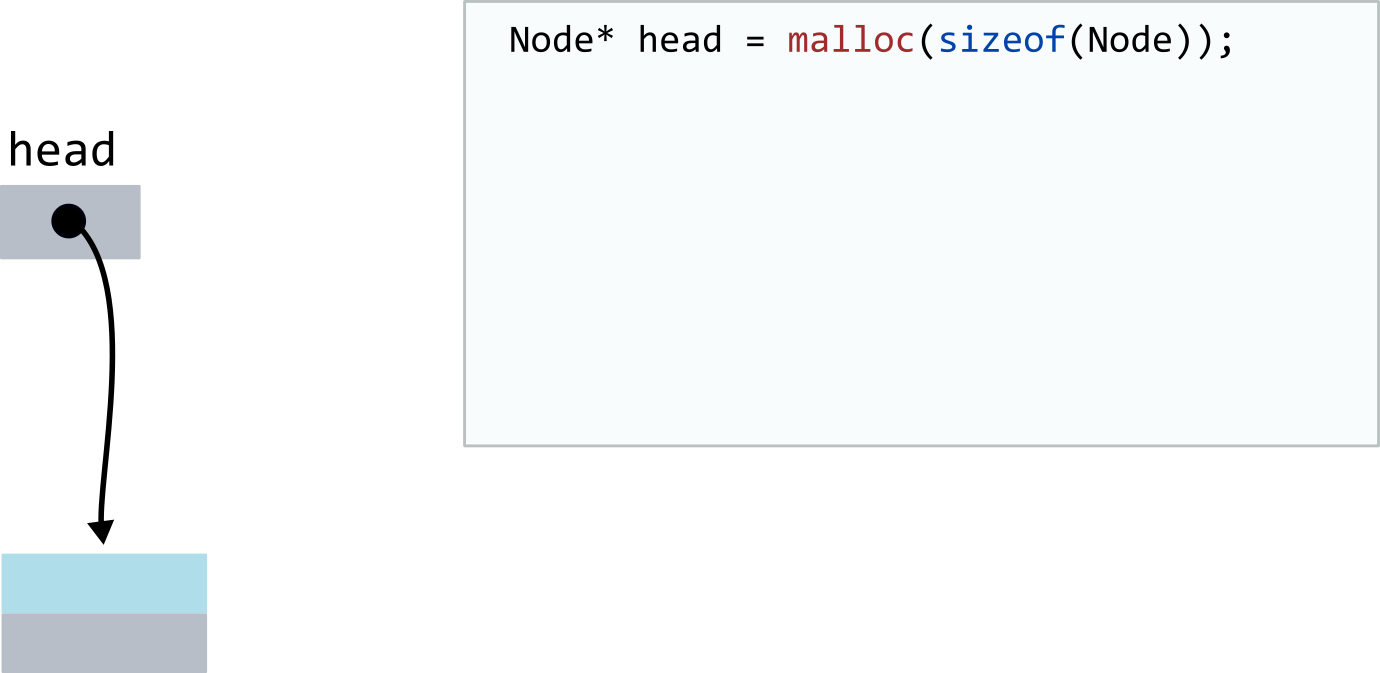
\includegraphics[width=\imageSizeMult\linewidth]{../images/codelist/codelist2.png}
\end{center}
\end{frame}


\begin{frame}[fragile]
\frametitle{Работа со связным списком}
\begin{center}
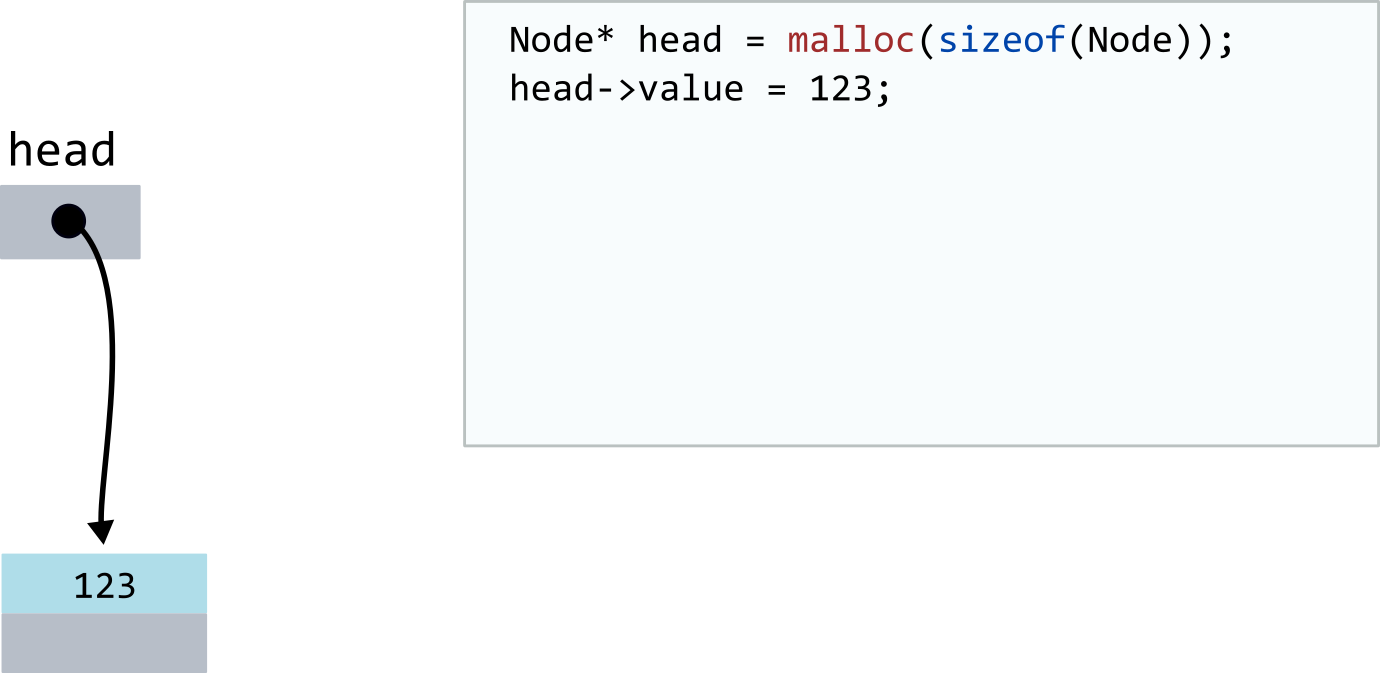
\includegraphics[width=\imageSizeMult\linewidth]{../images/codelist/codelist3.png}
\end{center}
\end{frame}


\begin{frame}[fragile]
\frametitle{Работа со связным списком}
\begin{center}
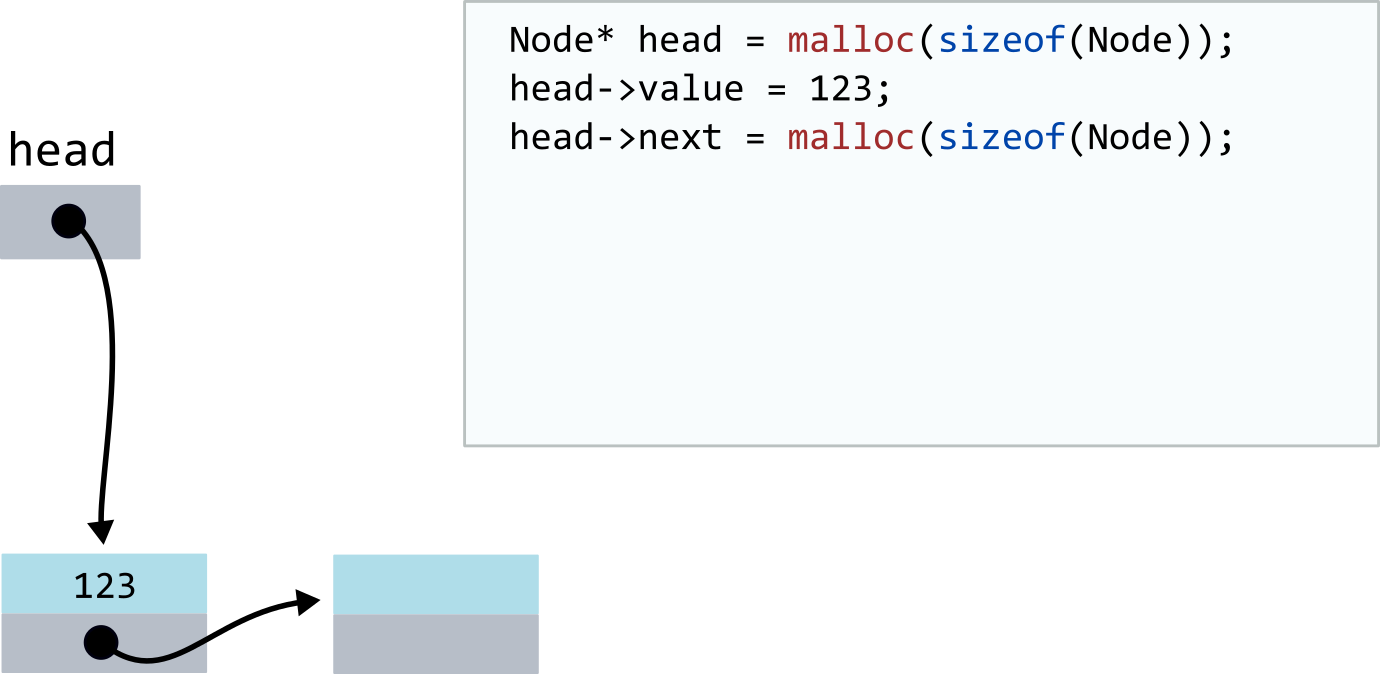
\includegraphics[width=\imageSizeMult\linewidth]{../images/codelist/codelist4.png}
\end{center}
\end{frame}


\begin{frame}[fragile]
\frametitle{Работа со связным списком}
\begin{center}
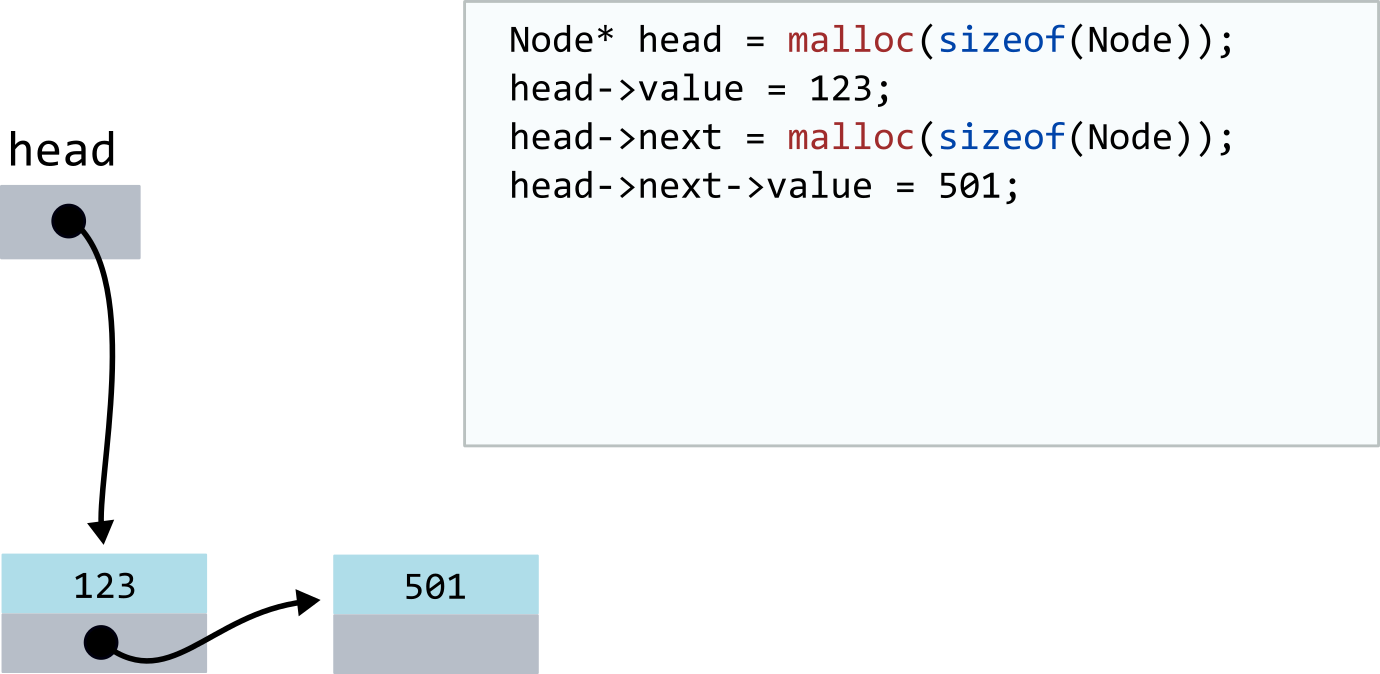
\includegraphics[width=\imageSizeMult\linewidth]{../images/codelist/codelist5.png}
\end{center}
\end{frame}


\begin{frame}[fragile]
\frametitle{Работа со связным списком}
\begin{center}
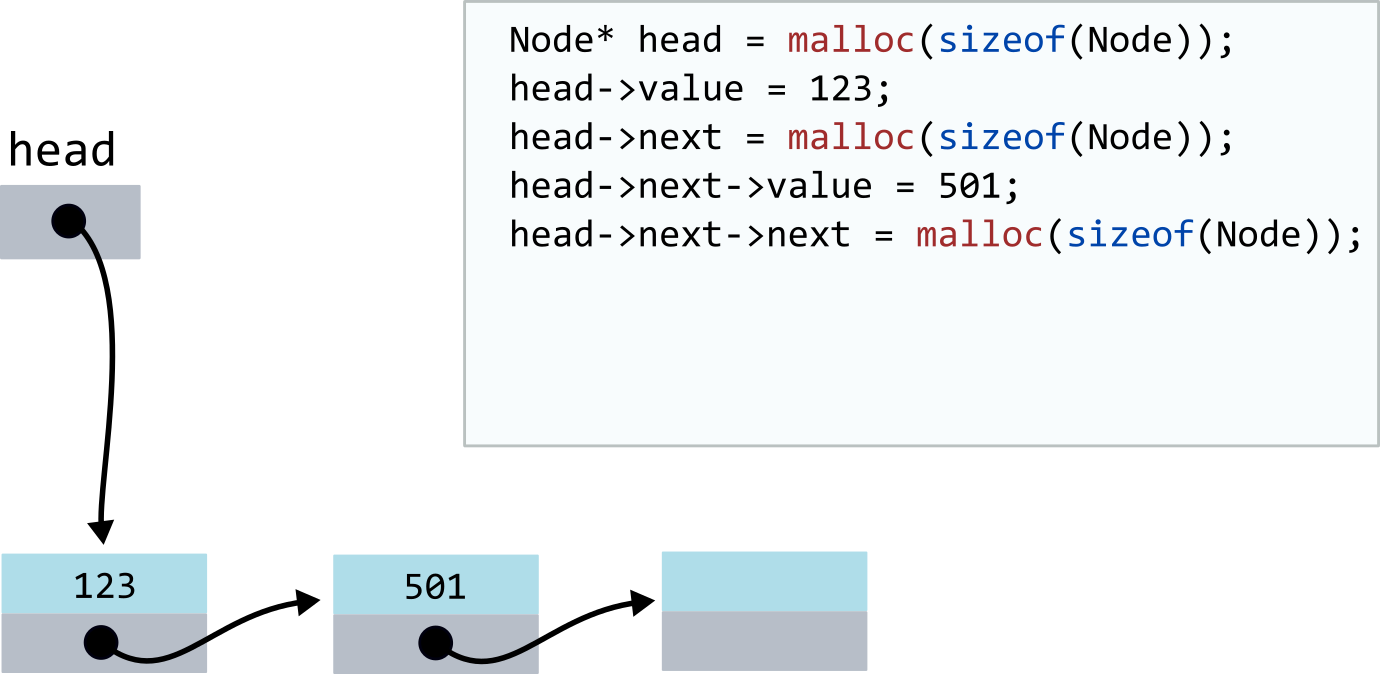
\includegraphics[width=\imageSizeMult\linewidth]{../images/codelist/codelist6.png}
\end{center}
\end{frame}


\begin{frame}[fragile]
\frametitle{Работа со связным списком}
\begin{center}
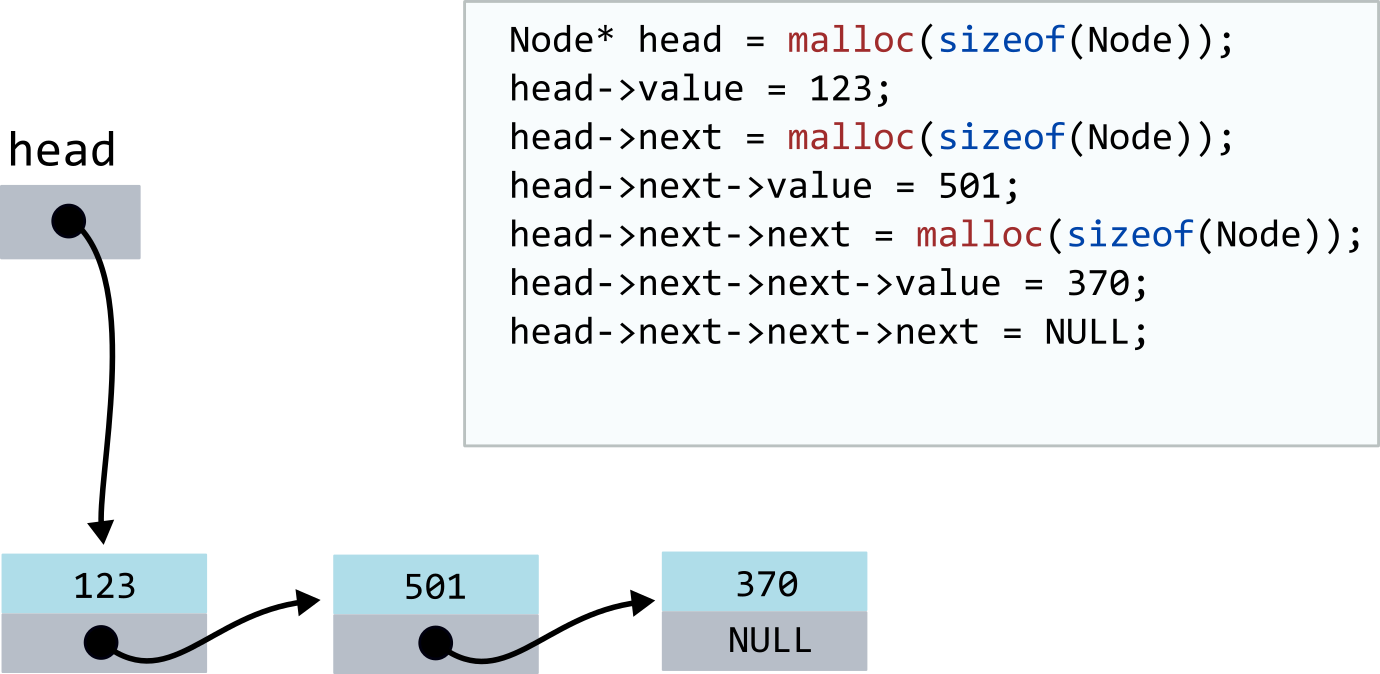
\includegraphics[width=\imageSizeMult\linewidth]{../images/codelist/codelist7.png}
\end{center}
\end{frame}


\section{Добавление элемента в конец связного списка}

\begin{frame}[fragile]
\frametitle{Добавление элемента в конец связного списка}
\begin{center}
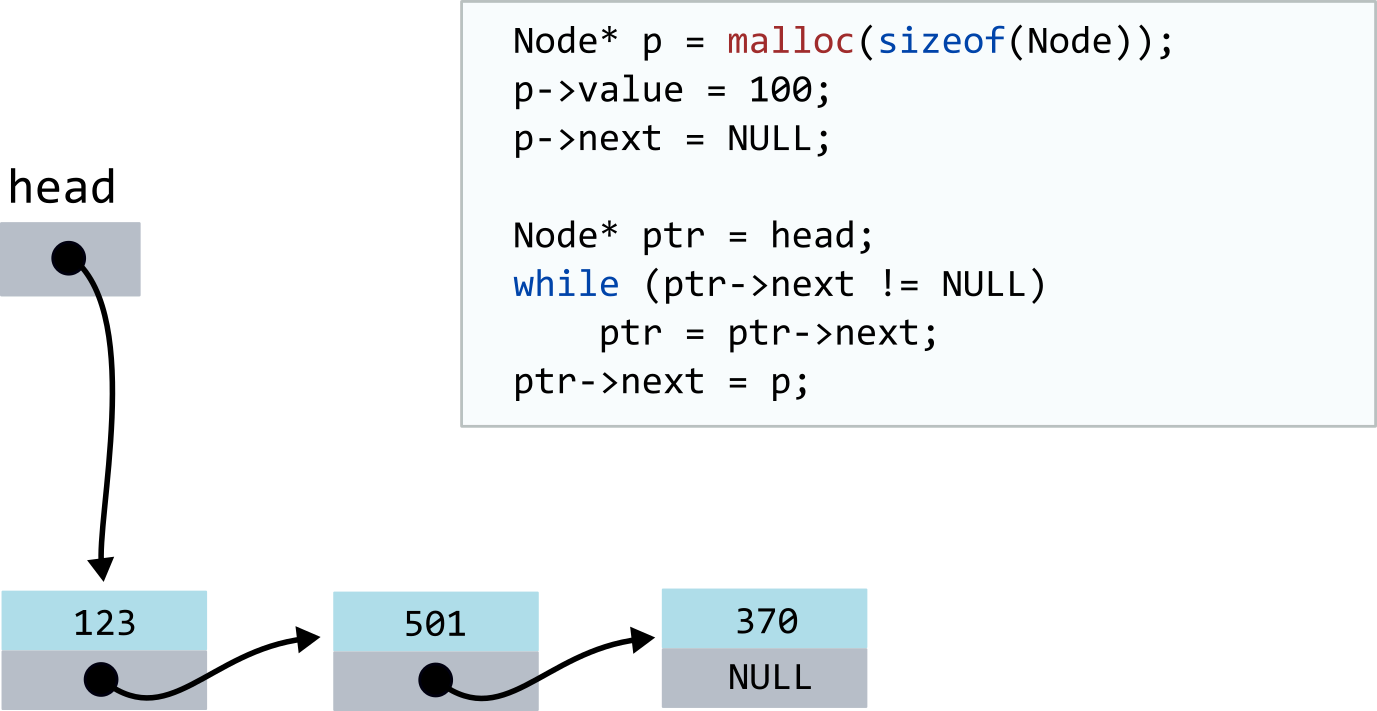
\includegraphics[width=\imageSizeMult\linewidth]{../images/codelist/codelistf_insert1.png}
\end{center}
\end{frame}


\begin{frame}[fragile]
\frametitle{Добавление элемента в конец связного списка}
\begin{center}
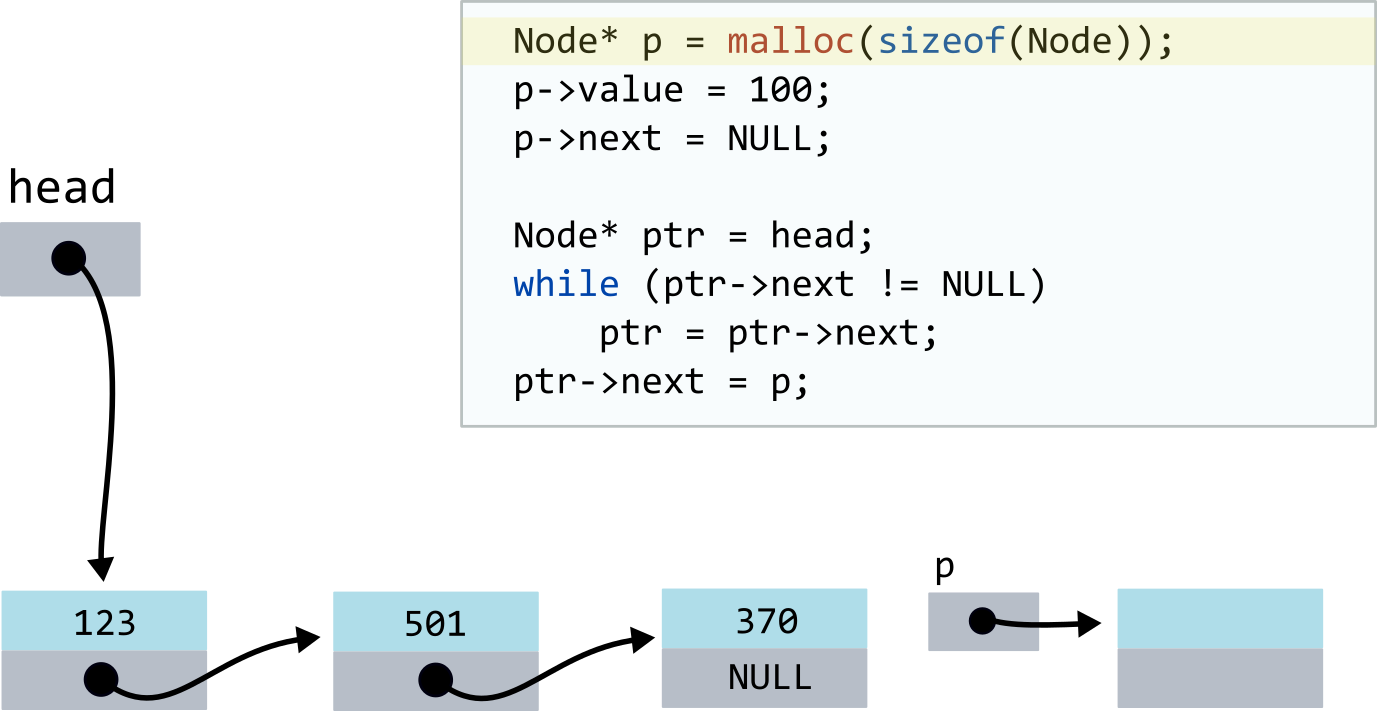
\includegraphics[width=\imageSizeMult\linewidth]{../images/codelist/codelistf_insert2.png}
\end{center}
\end{frame}



\begin{frame}[fragile]
\frametitle{Добавление элемента в конец связного списка}
\begin{center}
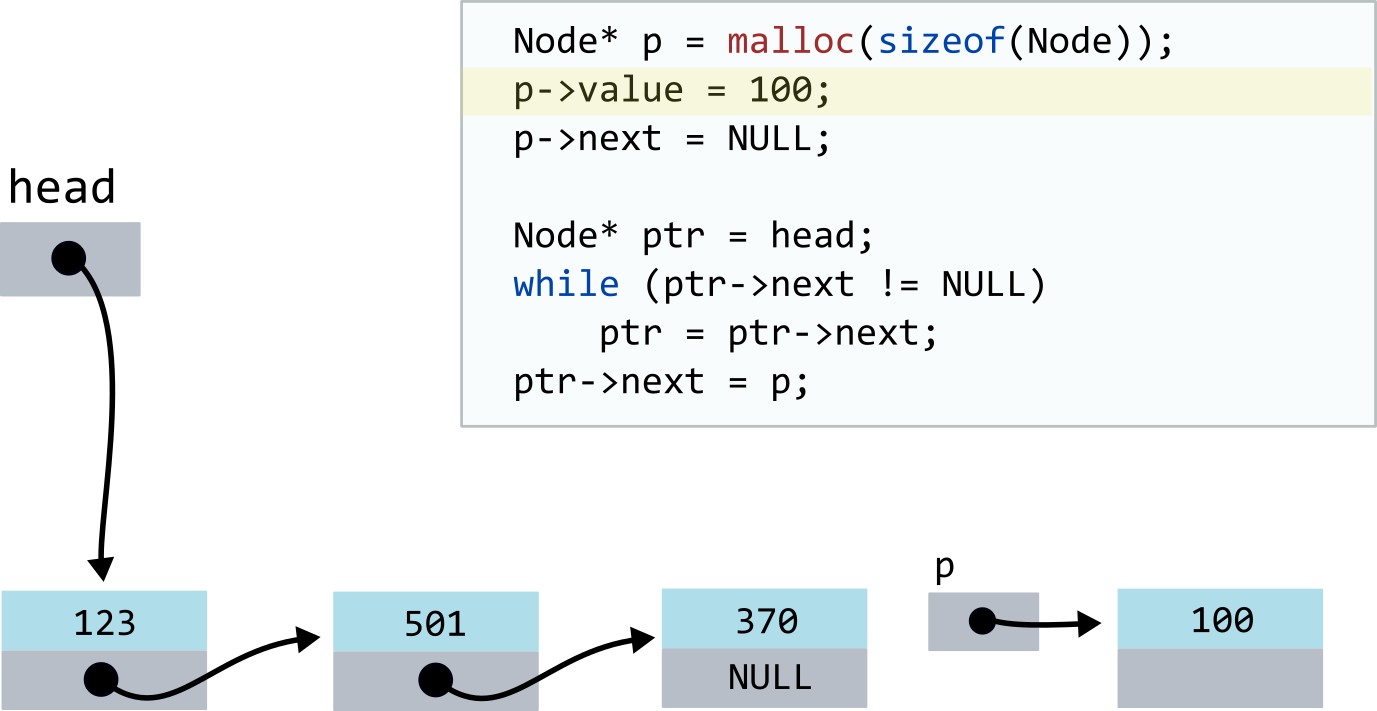
\includegraphics[width=\imageSizeMult\linewidth]{../images/codelist/codelistf_insert3.png}
\end{center}
\end{frame}



\begin{frame}[fragile]
\frametitle{Добавление элемента в конец связного списка}
\begin{center}
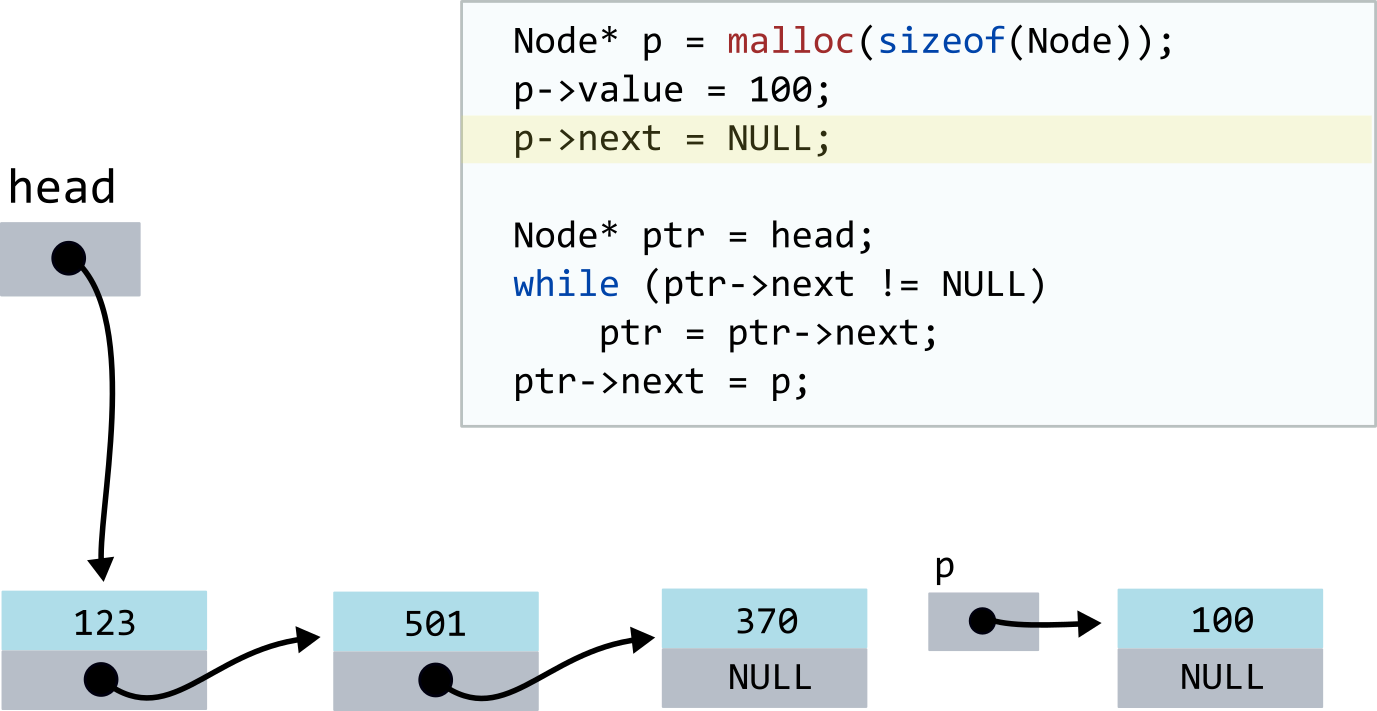
\includegraphics[width=\imageSizeMult\linewidth]{../images/codelist/codelistf_insert4.png}
\end{center}
\end{frame}



\begin{frame}[fragile]
\frametitle{Добавление элемента в конец связного списка}
\begin{center}
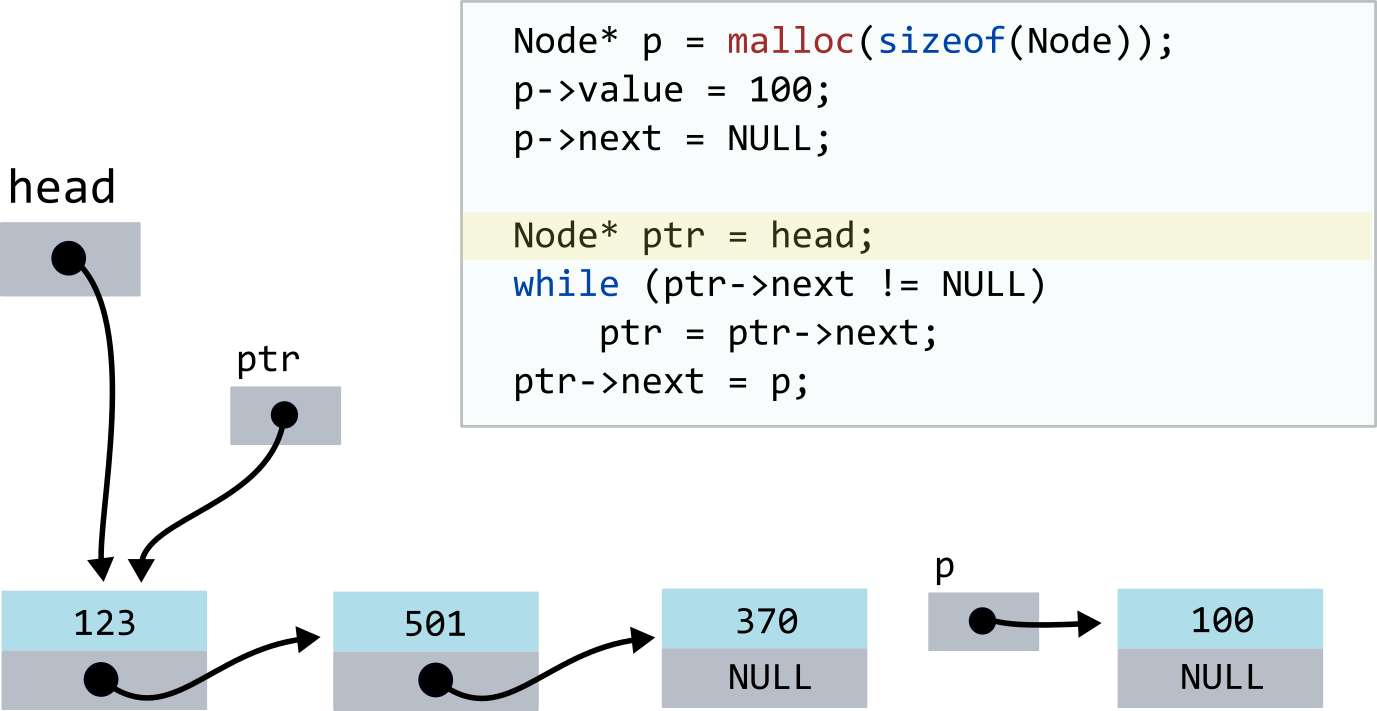
\includegraphics[width=\imageSizeMult\linewidth]{../images/codelist/codelistf_insert5.png}
\end{center}
\end{frame}



\begin{frame}[fragile]
\frametitle{Добавление элемента в конец связного списка}
\begin{center}
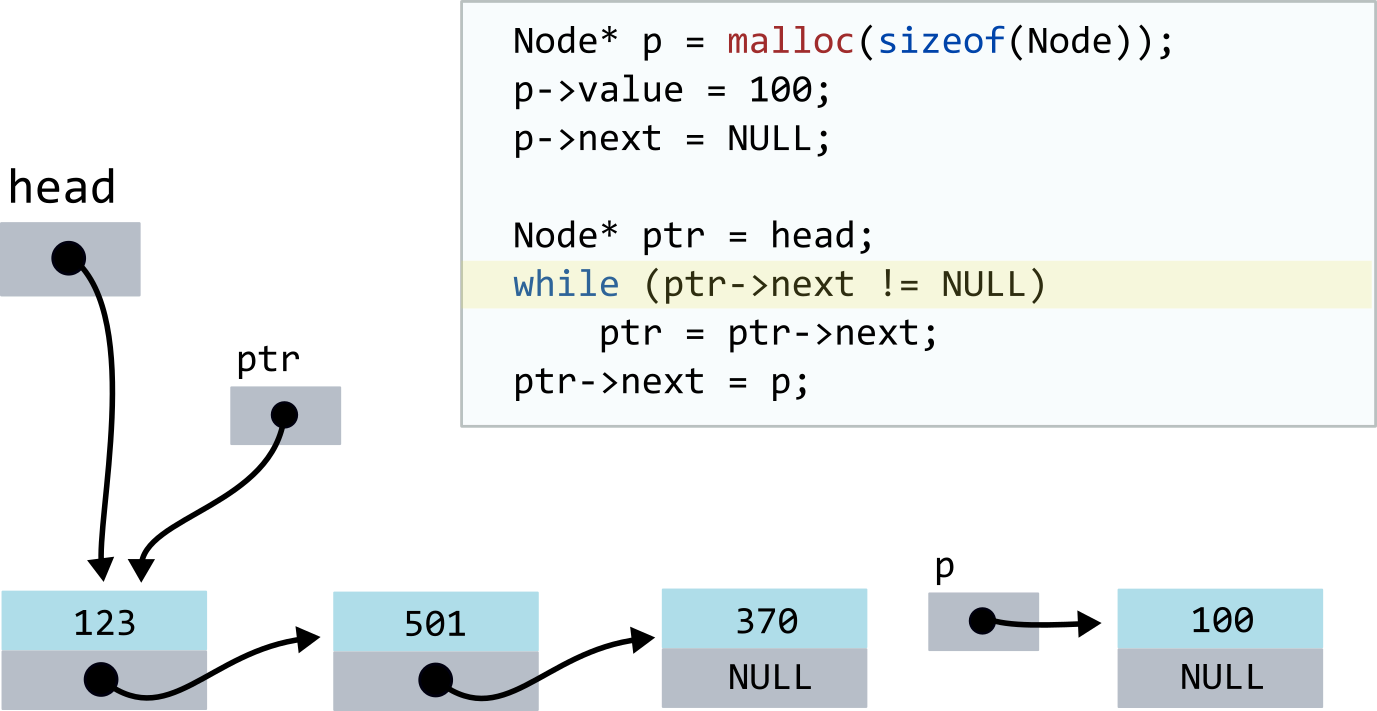
\includegraphics[width=\imageSizeMult\linewidth]{../images/codelist/codelistf_insert6.png}
\end{center}
\end{frame}



\begin{frame}[fragile]
\frametitle{Добавление элемента в конец связного списка}
\begin{center}
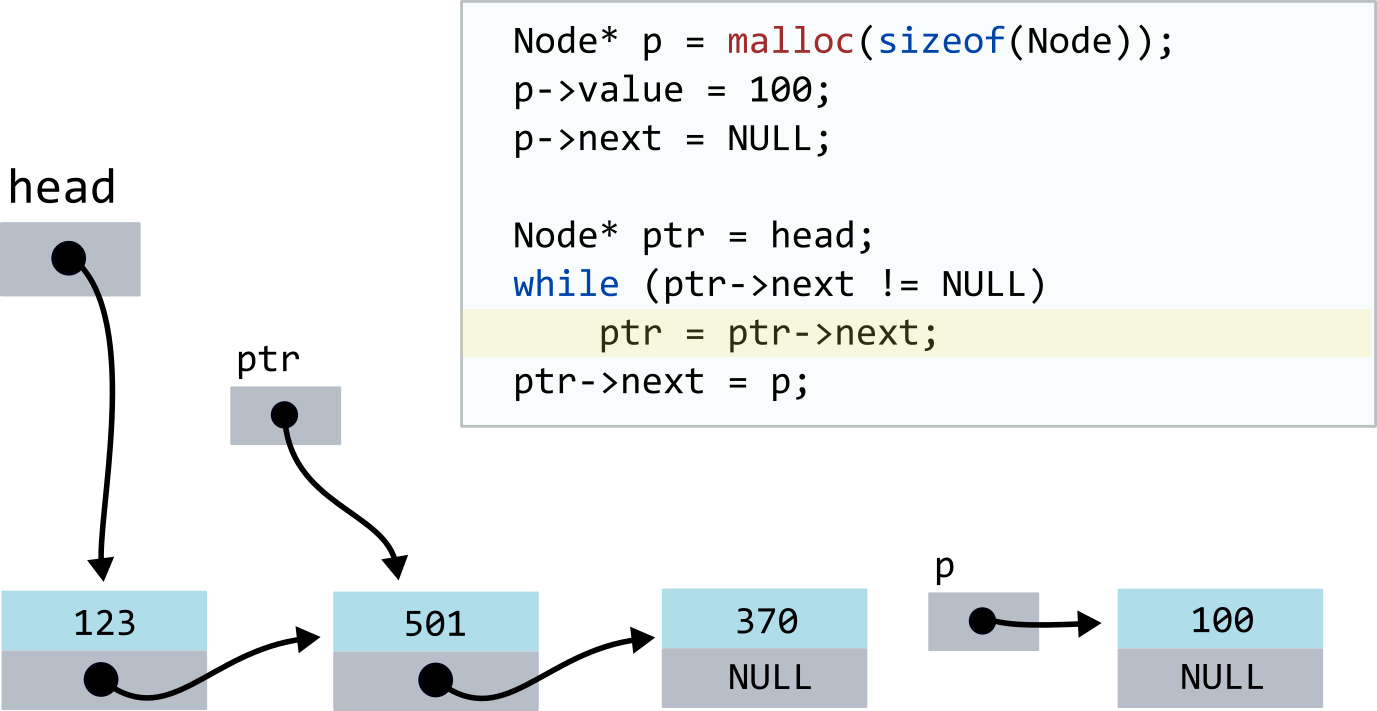
\includegraphics[width=\imageSizeMult\linewidth]{../images/codelist/codelistf_insert7.png}
\end{center}
\end{frame}



\begin{frame}[fragile]
\frametitle{Добавление элемента в конец связного списка}
\begin{center}
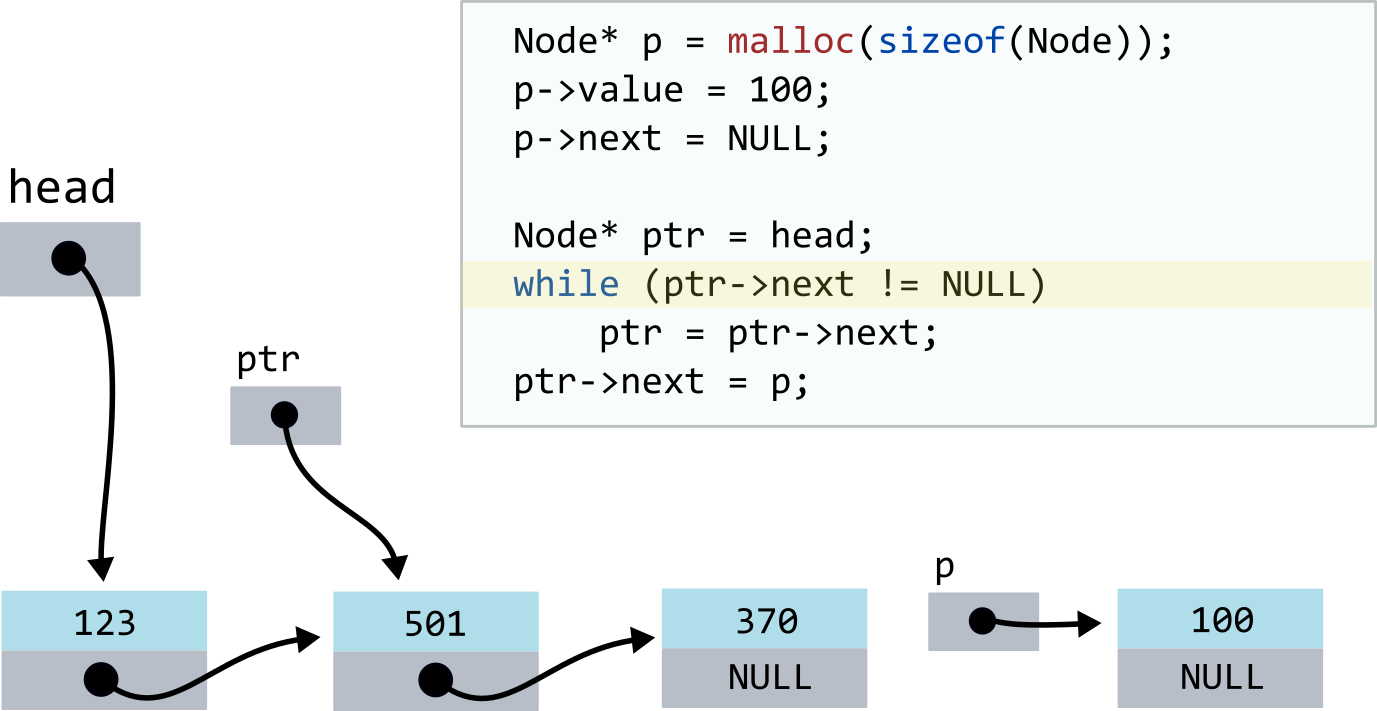
\includegraphics[width=\imageSizeMult\linewidth]{../images/codelist/codelistf_insert8.png}
\end{center}
\end{frame}



\begin{frame}[fragile]
\frametitle{Добавление элемента в конец связного списка}
\begin{center}
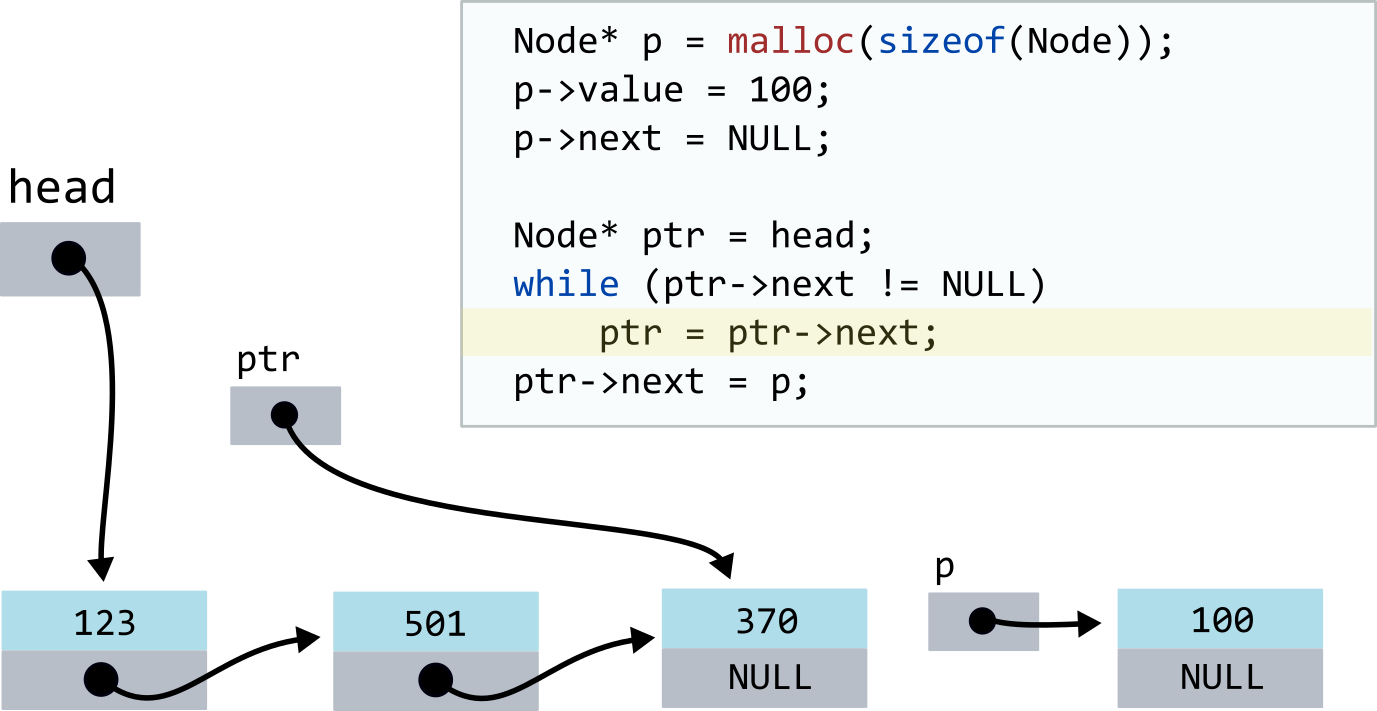
\includegraphics[width=\imageSizeMult\linewidth]{../images/codelist/codelistf_insert9.png}
\end{center}
\end{frame}



\begin{frame}[fragile]
\frametitle{Добавление элемента в конец связного списка}
\begin{center}
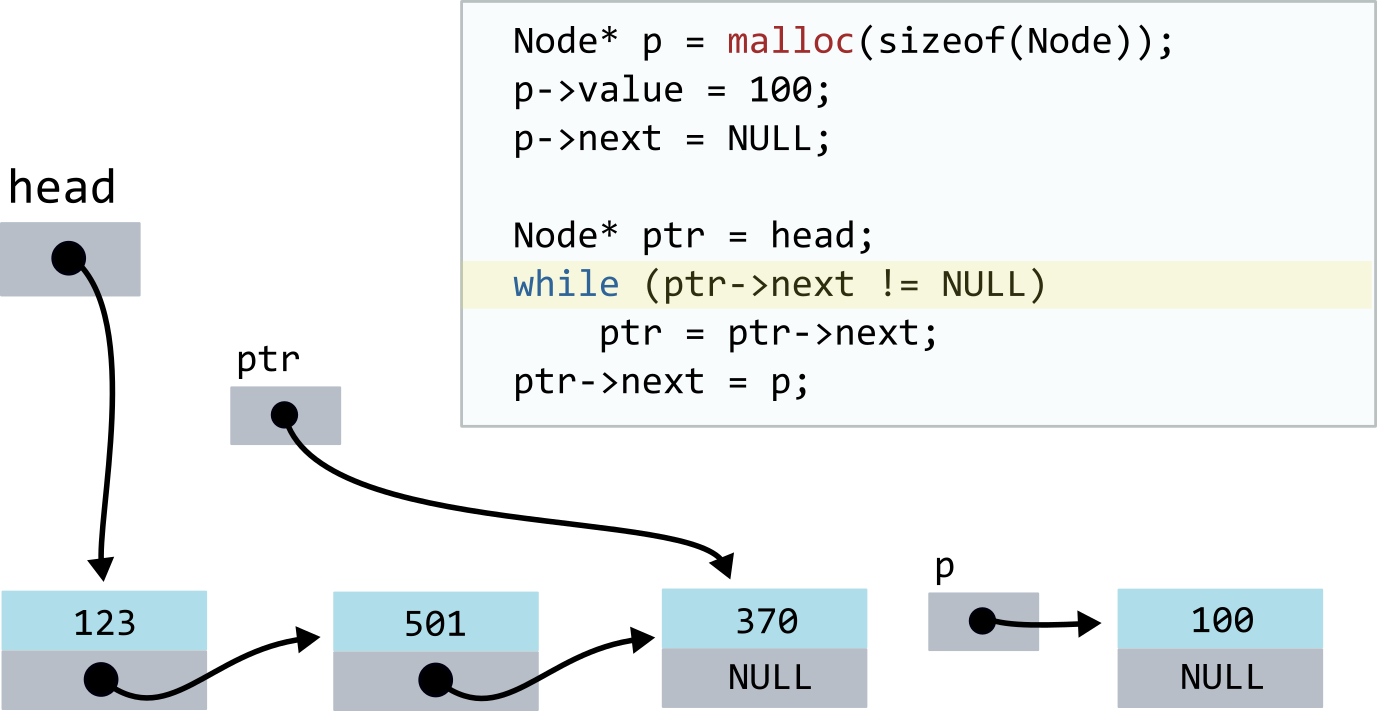
\includegraphics[width=\imageSizeMult\linewidth]{../images/codelist/codelistf_insert10.png}
\end{center}
\end{frame}



\begin{frame}[fragile]
\frametitle{Добавление элемента в конец связного списка}
\begin{center}
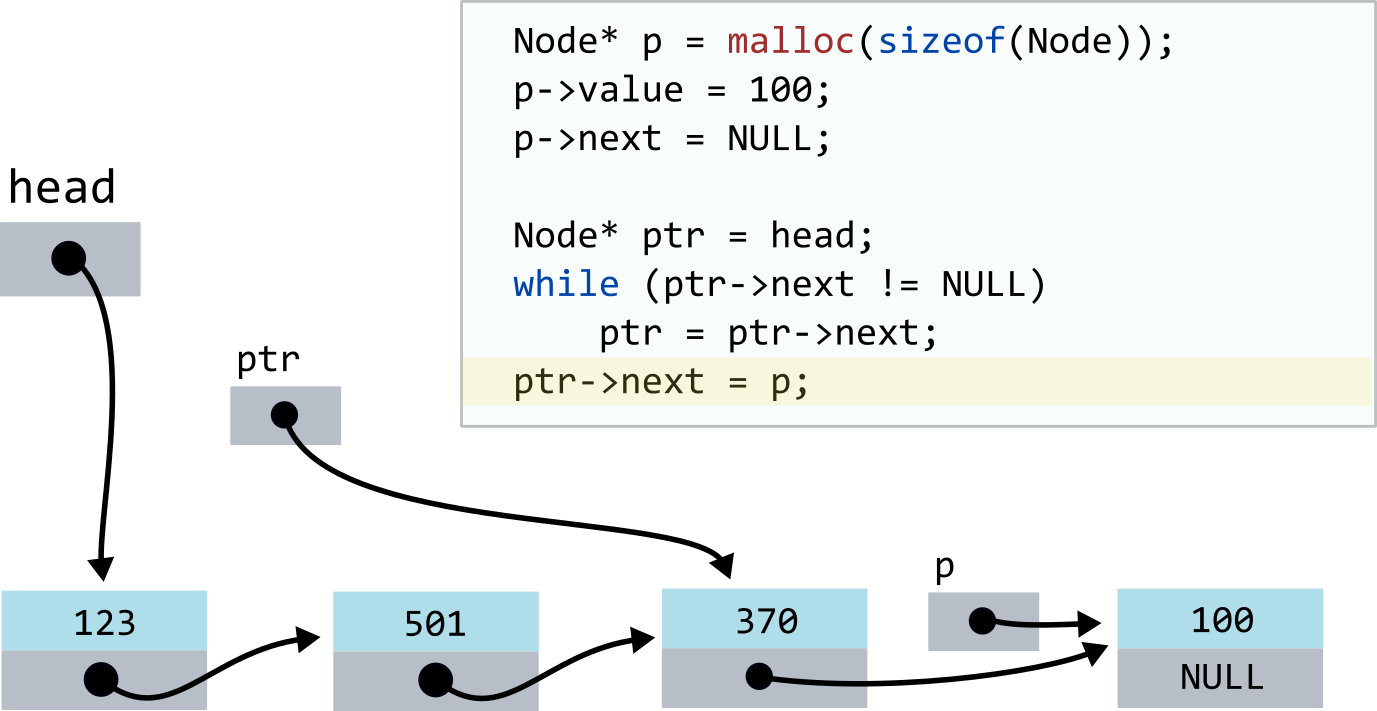
\includegraphics[width=\imageSizeMult\linewidth]{../images/codelist/codelistf_insert11.png}
\end{center}
\end{frame}



\begin{frame}[fragile]
\frametitle{Добавление элемента в конец связного списка}
\begin{center}
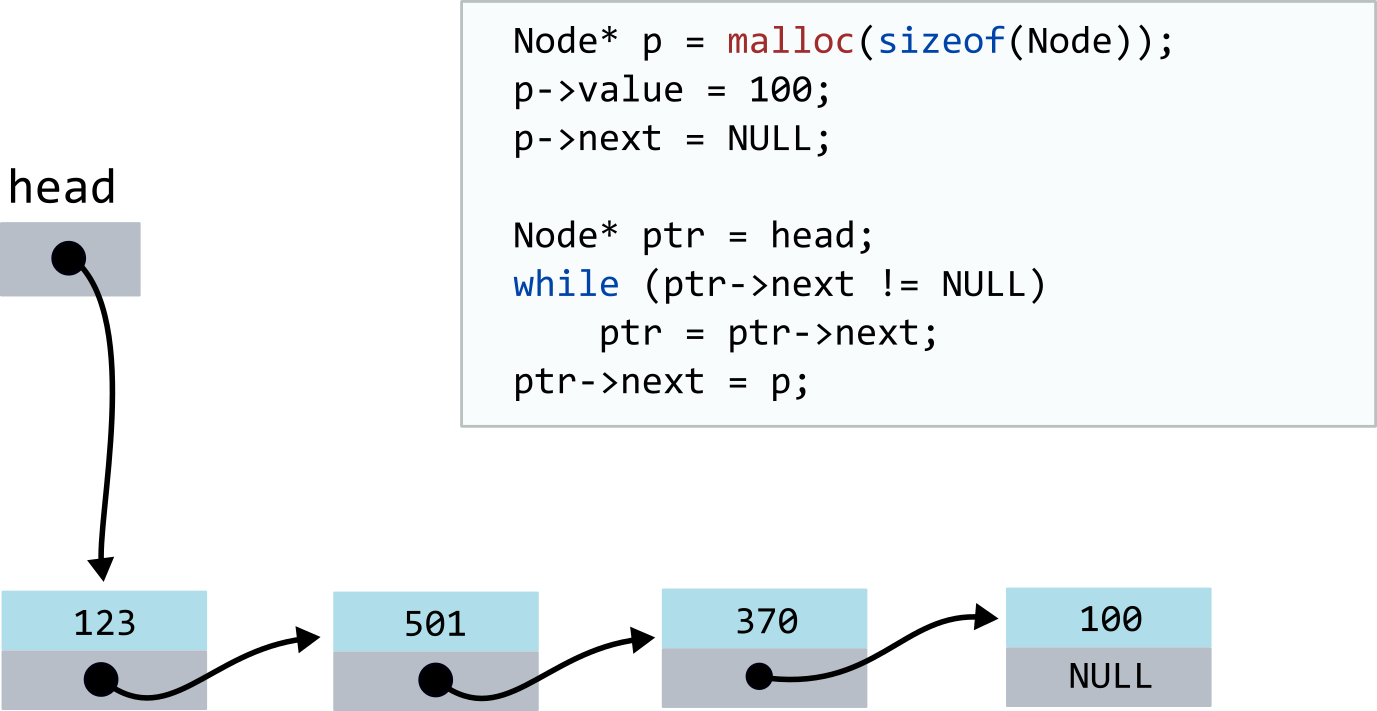
\includegraphics[width=\imageSizeMult\linewidth]{../images/codelist/codelistf_insert12.png}
\end{center}
\end{frame}


\section{Обращение связного списка}

\begin{frame}[fragile]
\frametitle{Обращение связного списка}
\begin{center}
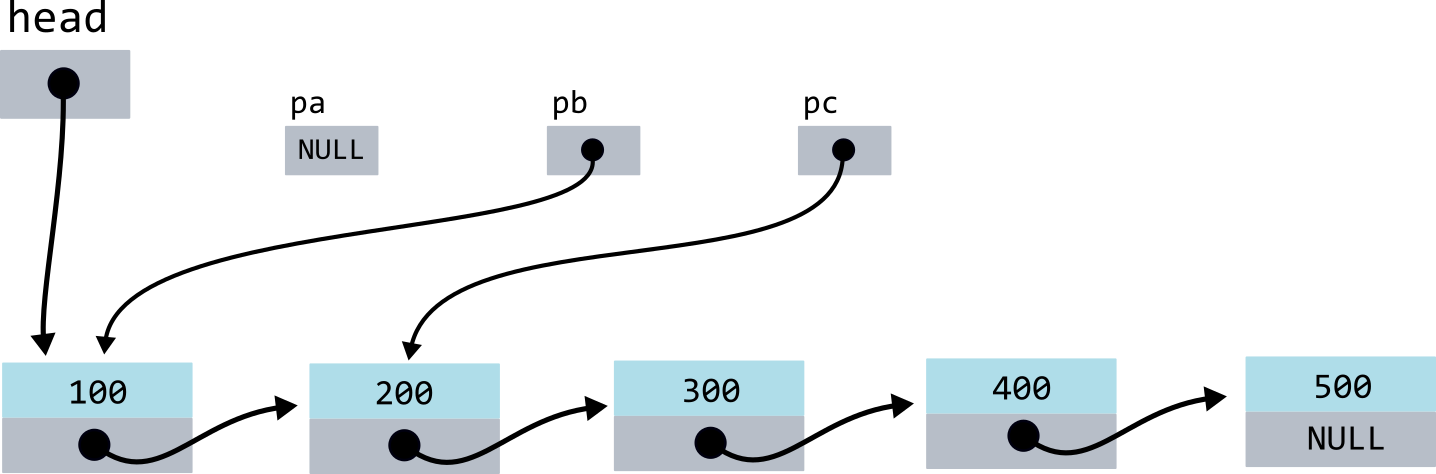
\includegraphics[width=\imageSizeMult\linewidth]{../images/reverse_list/reverse_list1.png}
\end{center}
\end{frame}

\begin{frame}[fragile]
\frametitle{Обращение связного списка}
\begin{center}
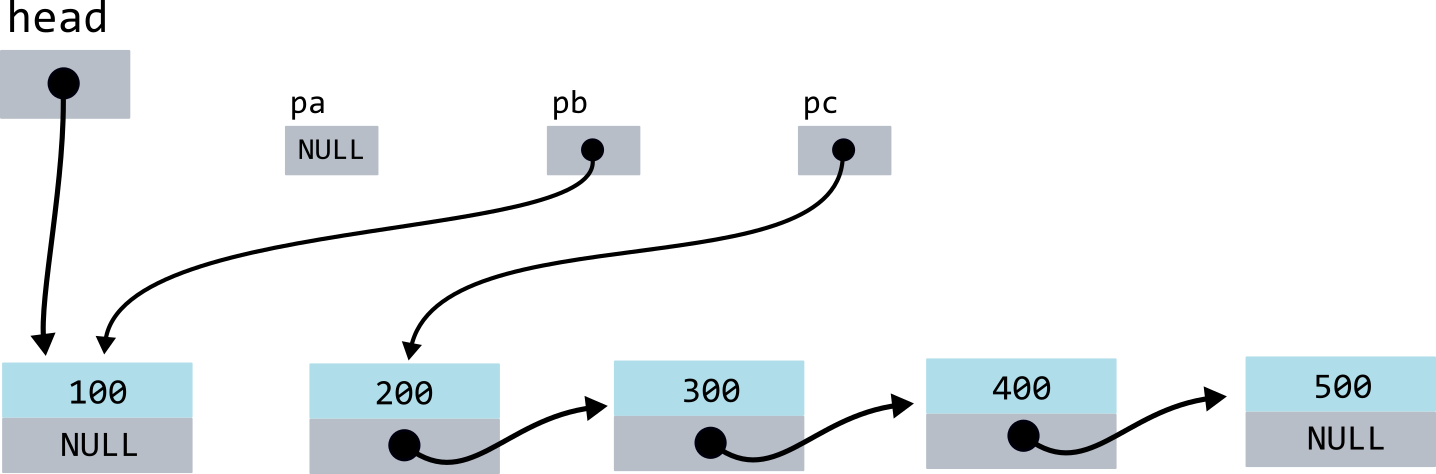
\includegraphics[width=\imageSizeMult\linewidth]{../images/reverse_list/reverse_list2.png}
\end{center}
\end{frame}

\begin{frame}[fragile]
\frametitle{Обращение связного списка}
\begin{center}
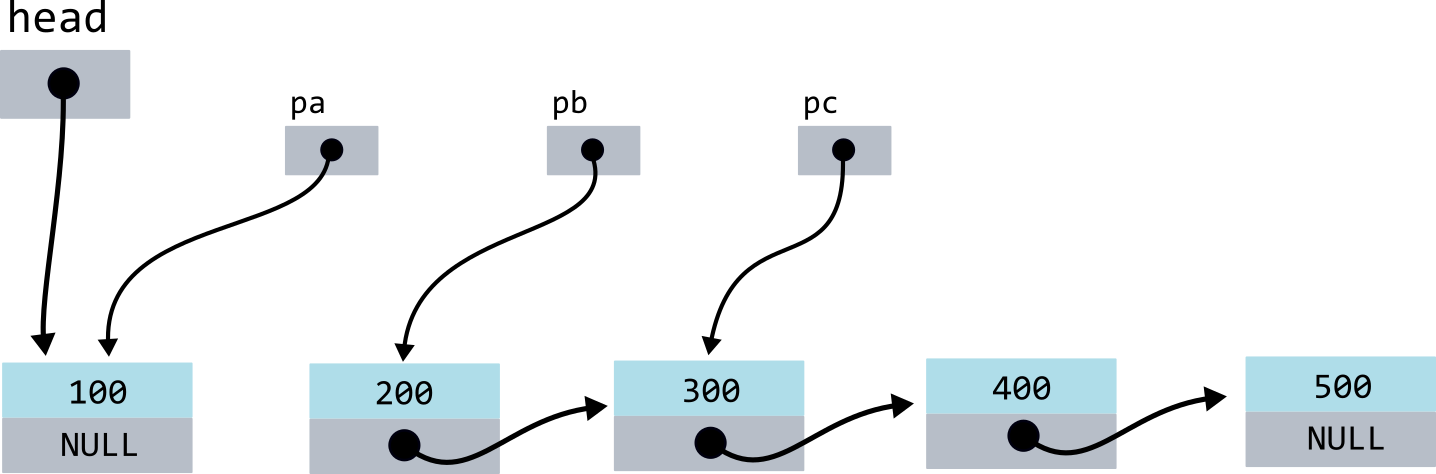
\includegraphics[width=\imageSizeMult\linewidth]{../images/reverse_list/reverse_list3.png}
\end{center}
\end{frame}

\begin{frame}[fragile]
\frametitle{Обращение связного списка}
\begin{center}
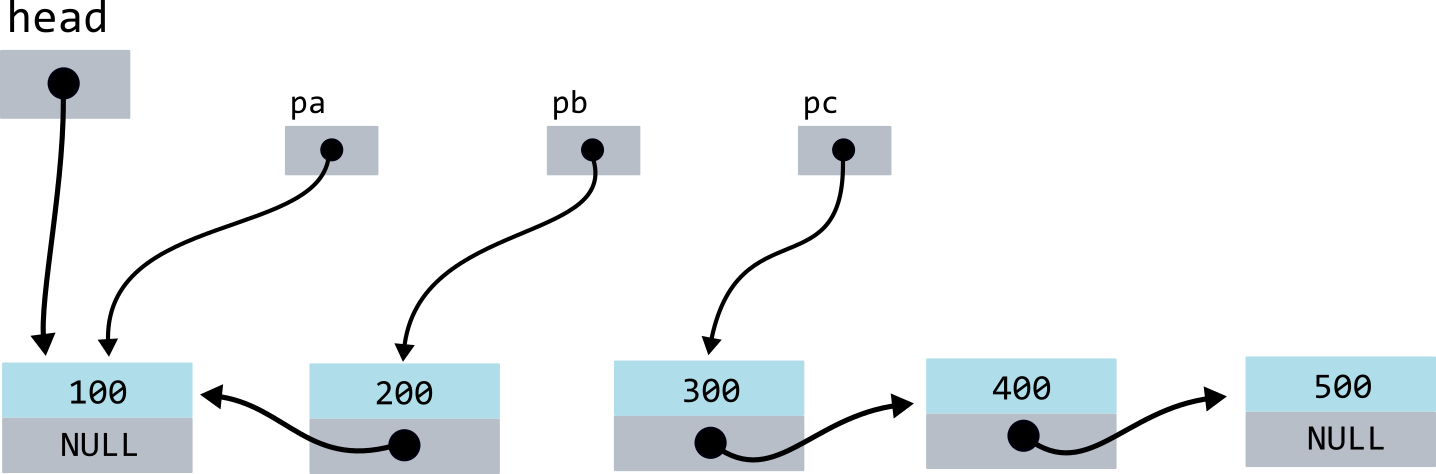
\includegraphics[width=\imageSizeMult\linewidth]{../images/reverse_list/reverse_list4.png}
\end{center}
\end{frame}

\begin{frame}[fragile]
\frametitle{Обращение связного списка}
\begin{center}
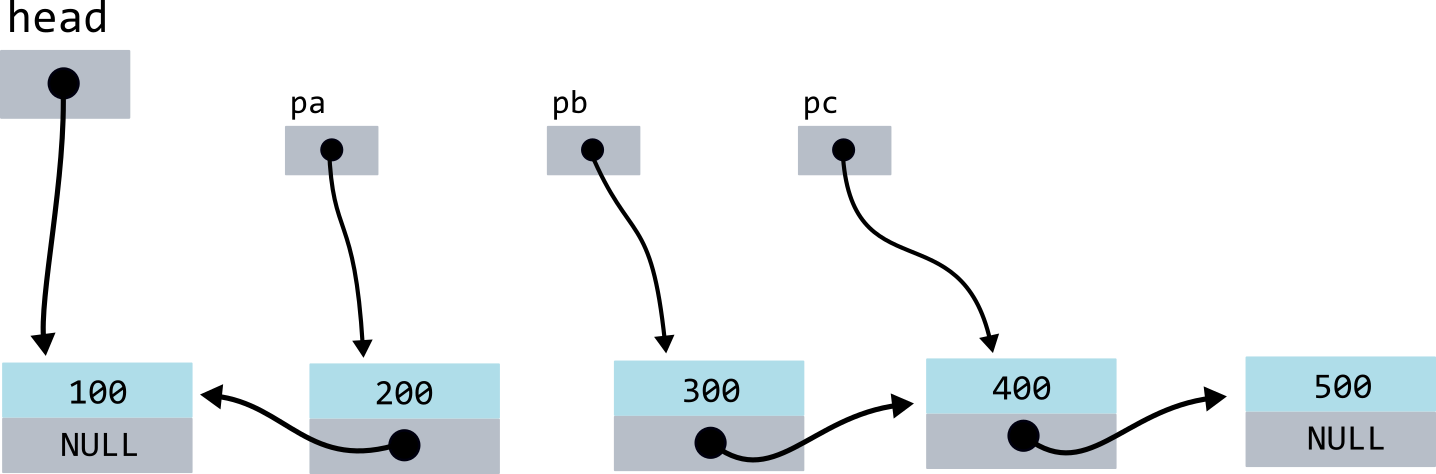
\includegraphics[width=\imageSizeMult\linewidth]{../images/reverse_list/reverse_list5.png}
\end{center}
\end{frame}

\begin{frame}[fragile]
\frametitle{Обращение связного списка}
\begin{center}
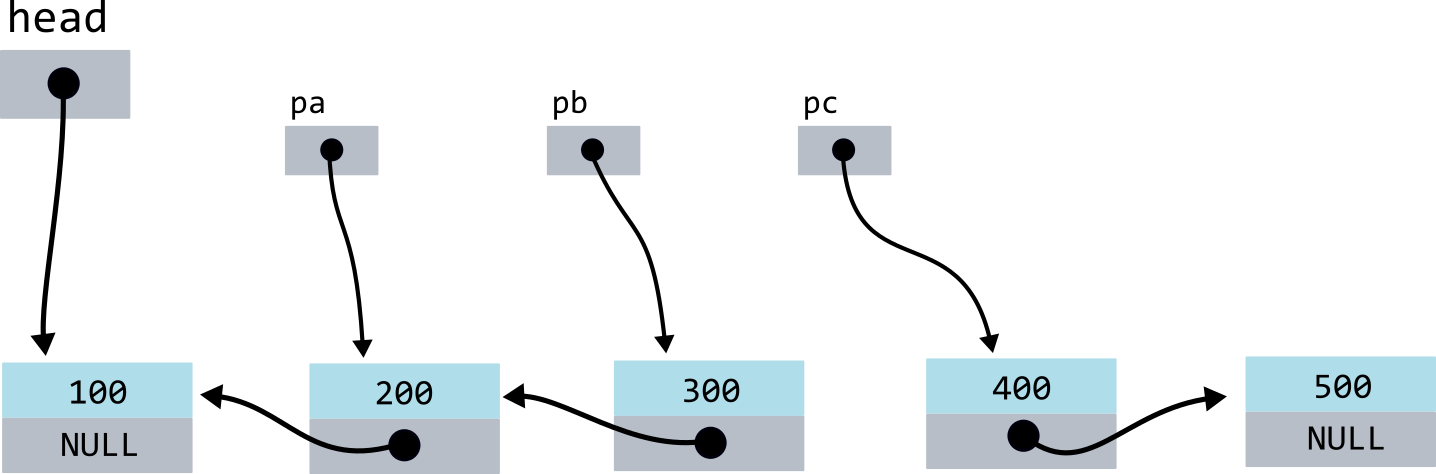
\includegraphics[width=\imageSizeMult\linewidth]{../images/reverse_list/reverse_list6.png}
\end{center}
\end{frame}

\begin{frame}[fragile]
\frametitle{Обращение связного списка}
\begin{center}
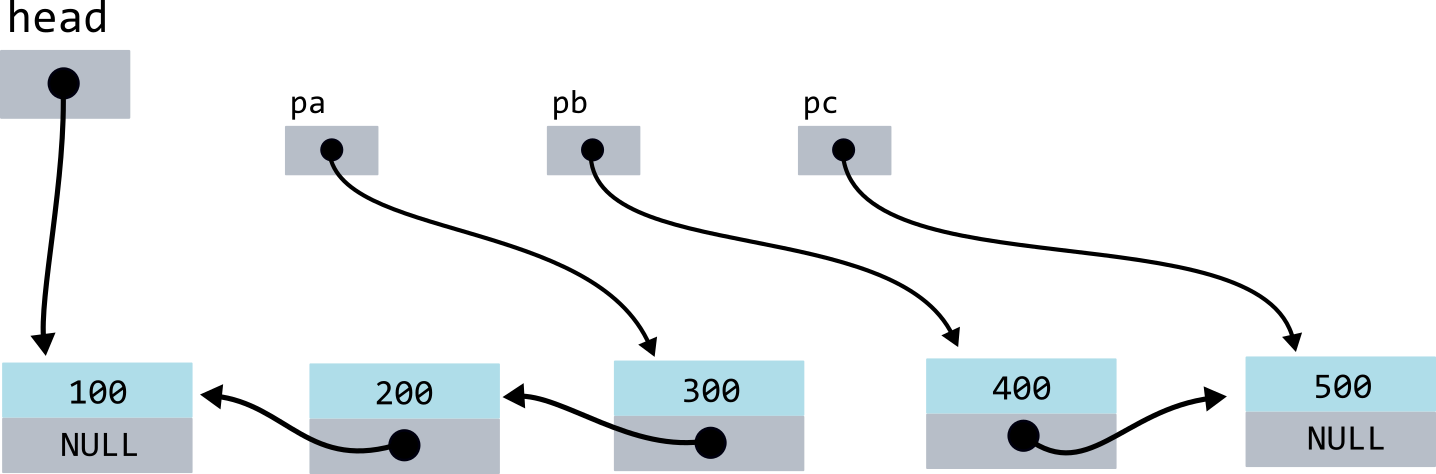
\includegraphics[width=\imageSizeMult\linewidth]{../images/reverse_list/reverse_list7.png}
\end{center}
\end{frame}

\begin{frame}[fragile]
\frametitle{Обращение связного списка}
\begin{center}
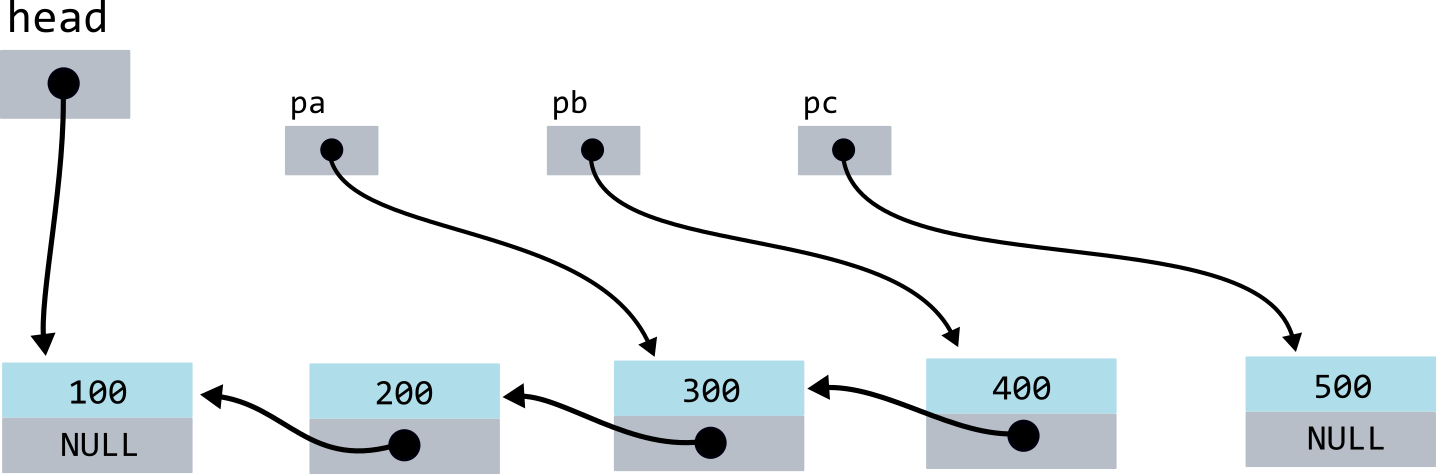
\includegraphics[width=\imageSizeMult\linewidth]{../images/reverse_list/reverse_list8.png}
\end{center}
\end{frame}

\begin{frame}[fragile]
\frametitle{Обращение связного списка}
\begin{center}
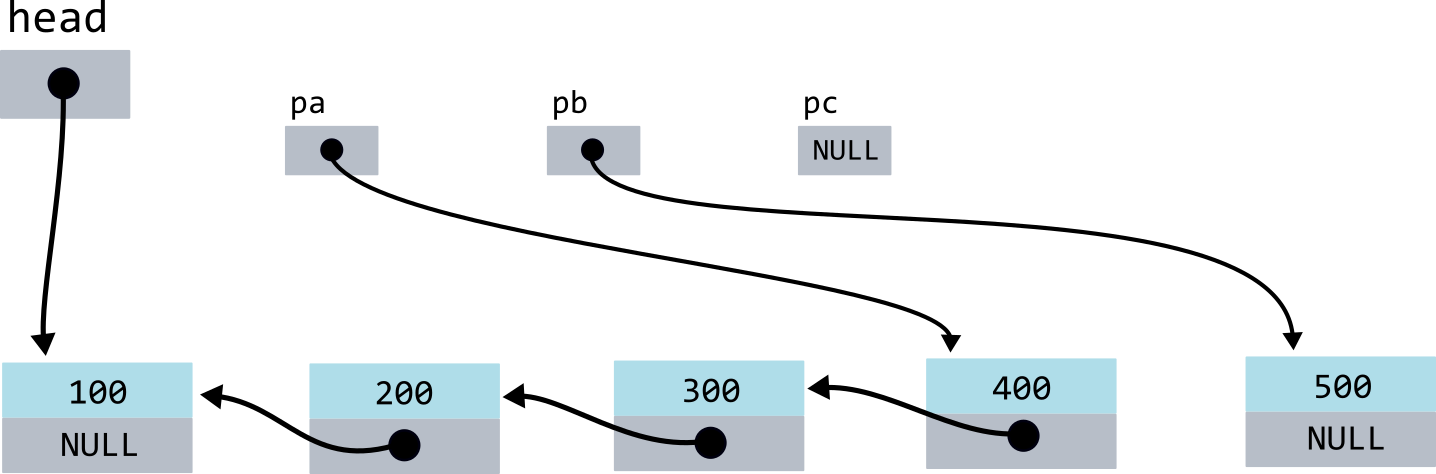
\includegraphics[width=\imageSizeMult\linewidth]{../images/reverse_list/reverse_list9.png}
\end{center}
\end{frame}

\begin{frame}[fragile]
\frametitle{Обращение связного списка}
\begin{center}
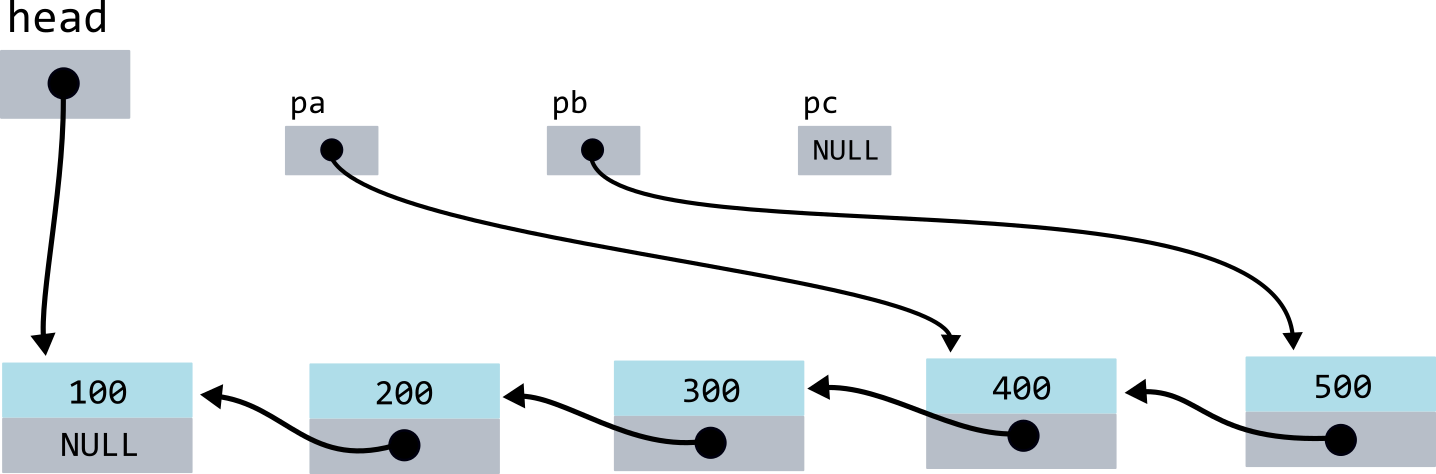
\includegraphics[width=\imageSizeMult\linewidth]{../images/reverse_list/reverse_list10.png}
\end{center}
\end{frame}

\begin{frame}[fragile]
\frametitle{Обращение связного списка}
\begin{center}
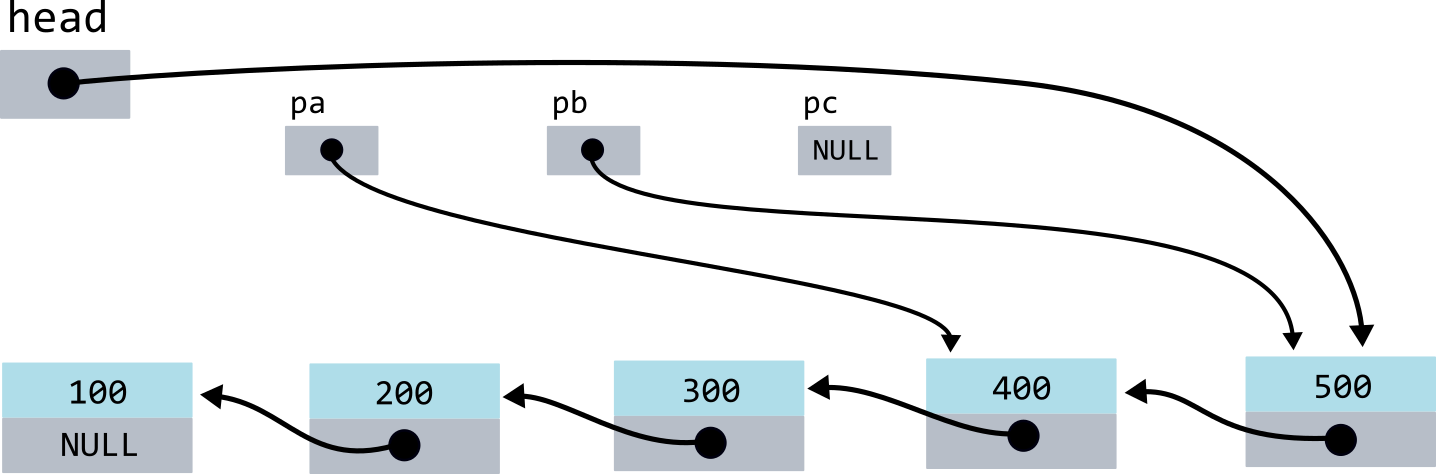
\includegraphics[width=\imageSizeMult\linewidth]{../images/reverse_list/reverse_list11.png}
\end{center}
\end{frame}

\section{Вычислительная сложность операций со связным списком}
\begin{frame}[fragile]
\frametitle{Вычислительная сложность операций со связным списком}
\begin{center}
\begin{tabular}{ c c c }
 Операция & Массив & Односвязный список \\ 
 \hline
 Доступ по номеру & $O(1)$ & $O(N)$  \\
 Поиск & $O(N)$ & $O(N)$  \\    
 Вставка в начало & $O(N)$ & $O(1)$  \\
 Вставка в конец & $O(1)$ & $O(N)$  \\
 \begin{tabular}{@{}c@{}}Вставка в конец если известен \\ указатель на последний элемент\end{tabular} & $O(1)$ & $O(1)$  \\
 Вставка в середину & $O(N)$ & $O(N)$  \\
 \begin{tabular}{@{}c@{}}Вставка в середину если известен \\ указатель на предыдущий элемент\end{tabular} & $O(N)$ & $O(1)$  \\  
\end{tabular}
\end{center}
\end{frame}

\begin{frame}[fragile]
\frametitle{Недостатки связного списка}
\begin{itemize}
\item В отличии от массива долгий доступ по индексу ($O(N)$)
\item Чтобы вставить в конец списка, нужно пробежать до конца списка, а это долго ($O(N)$)
\item С удаление из конца списка то же самое ($O(N)$)
\item Если известен указатель на элемент списка, то можно быстро вставить элемент после него, но нельзя быстро вставить элемент до него (только за $O(N)$).
\item Если известен указатель на элемент списка, то нельзя быстро удалить его, так как нужно знать указатель на предыдущий элемент.
\end{itemize}
Двусвязный список решает эти недостатки (кроме долгого доступа по индексу)
\end{frame}
\section{Двусвязный список}

\begin{frame}[fragile]
\frametitle{Двусвязный список: Определение}
\begin{center}
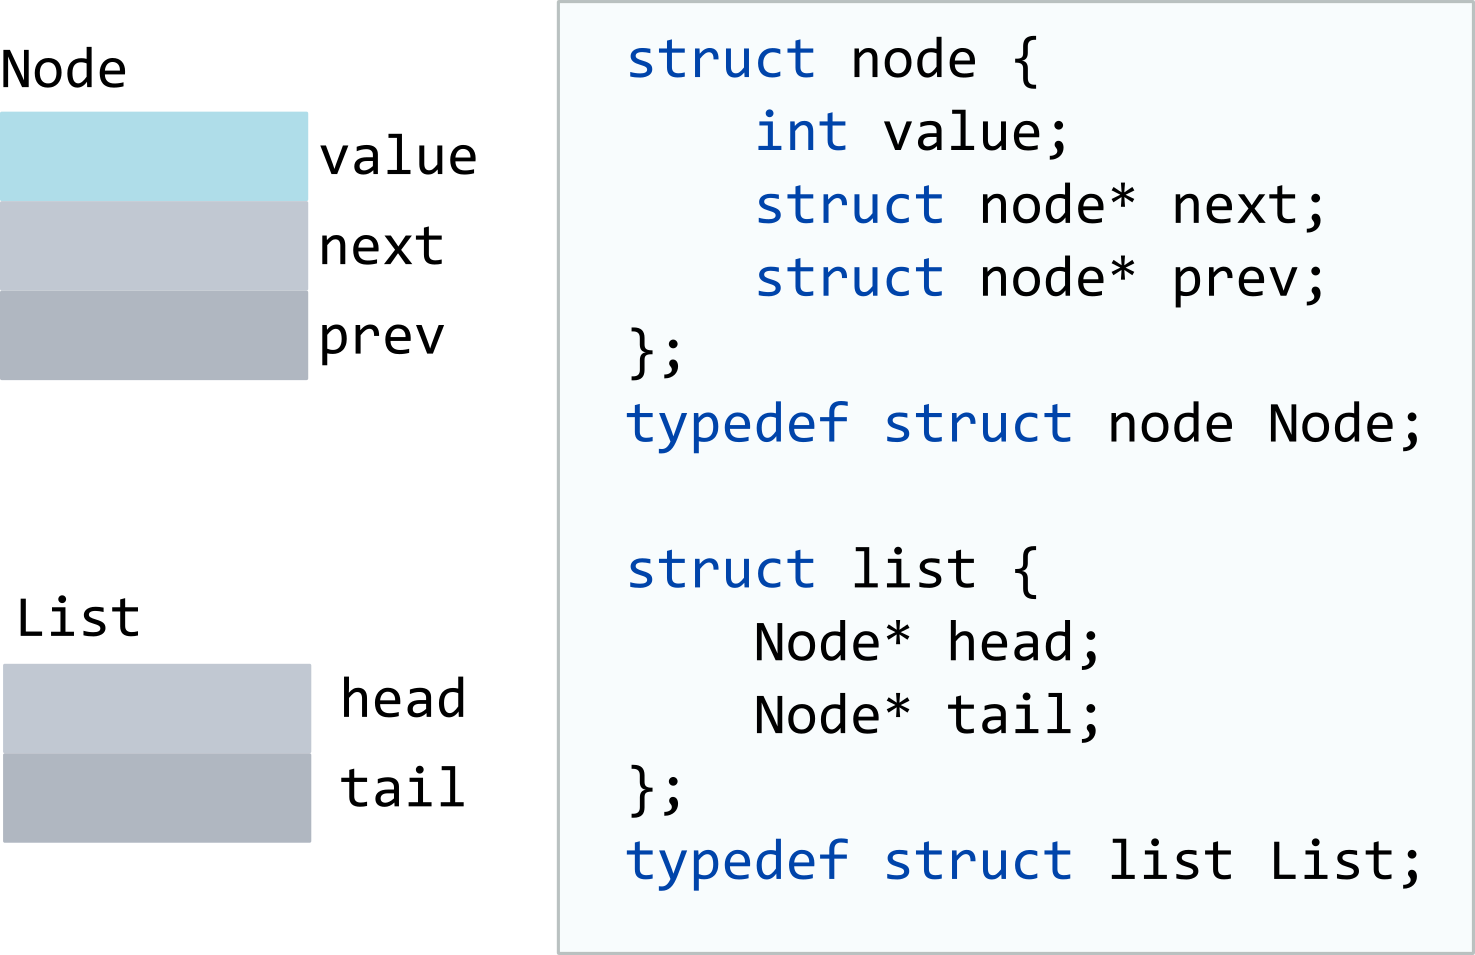
\includegraphics[width=\imageSizeMult\linewidth]{../images/doublylist/doublylist_definition.png}
\end{center}
\end{frame}

\section{Добавление элемент в конец двусвязного списка}

\begin{frame}[fragile]
\frametitle{Добавление элемент в конец двусвязного списка}
\begin{center}
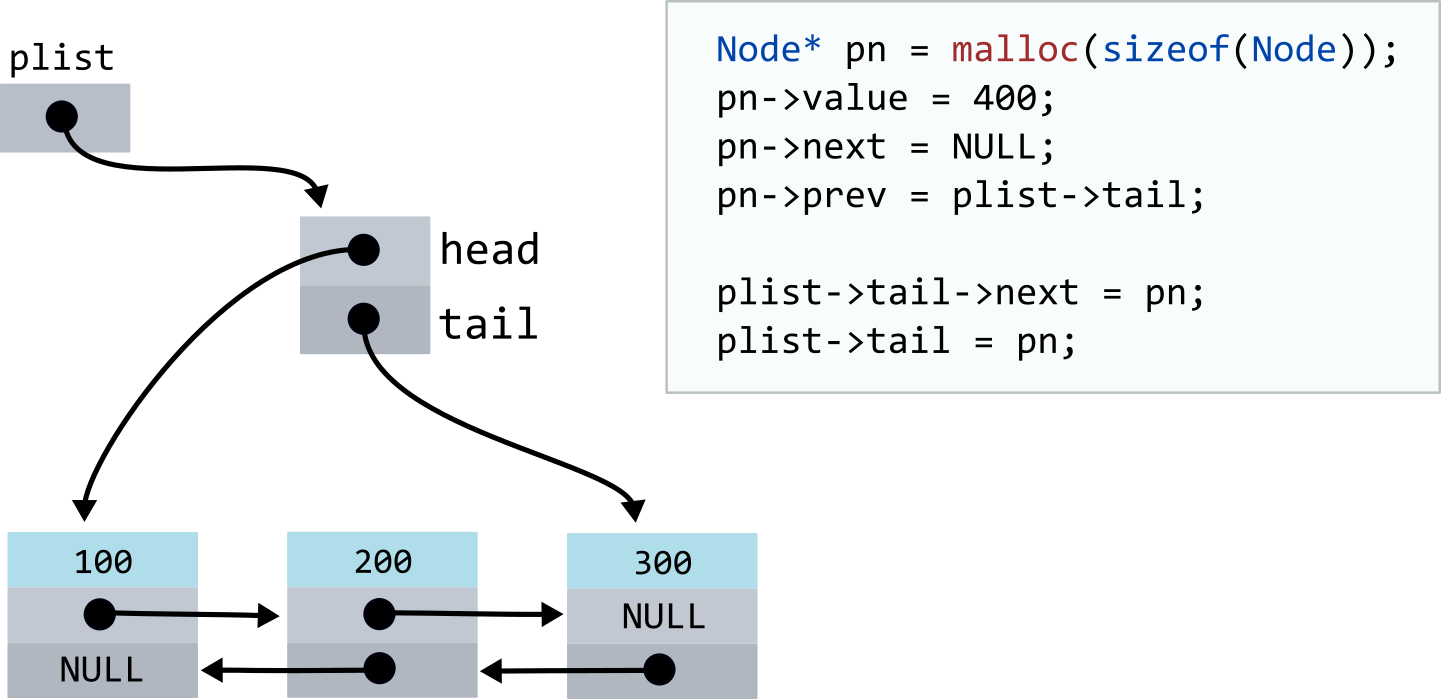
\includegraphics[width=\imageSizeMult\linewidth]{../images/doublylist/doublylist_addlast1.png}
\end{center}
\end{frame}

\begin{frame}[fragile]
\frametitle{Добавление элемент в конец двусвязного списка}
\begin{center}
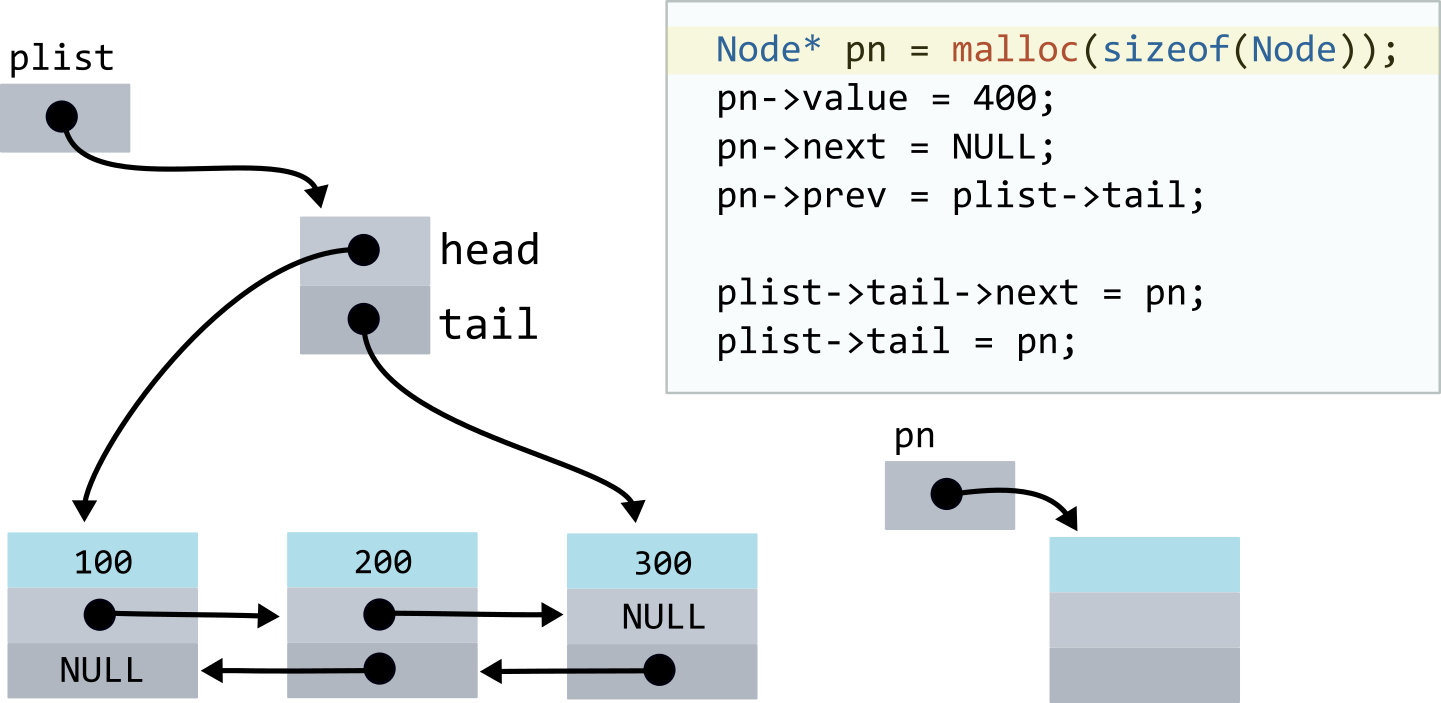
\includegraphics[width=\imageSizeMult\linewidth]{../images/doublylist/doublylist_addlast2.png}
\end{center}
\end{frame}

\begin{frame}[fragile]
\frametitle{Добавление элемент в конец двусвязного списка}
\begin{center}
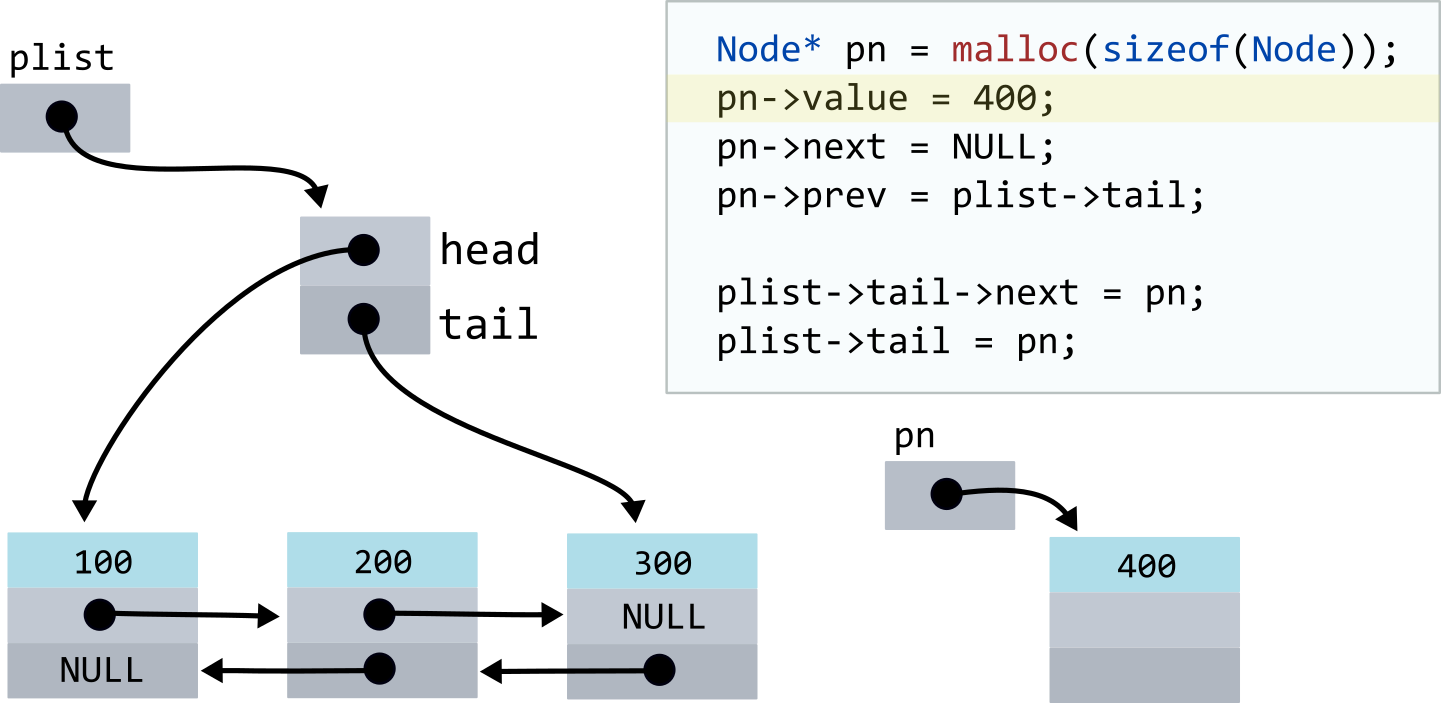
\includegraphics[width=\imageSizeMult\linewidth]{../images/doublylist/doublylist_addlast3.png}
\end{center}
\end{frame}


\begin{frame}[fragile]
\frametitle{Добавление элемент в конец двусвязного списка}
\begin{center}
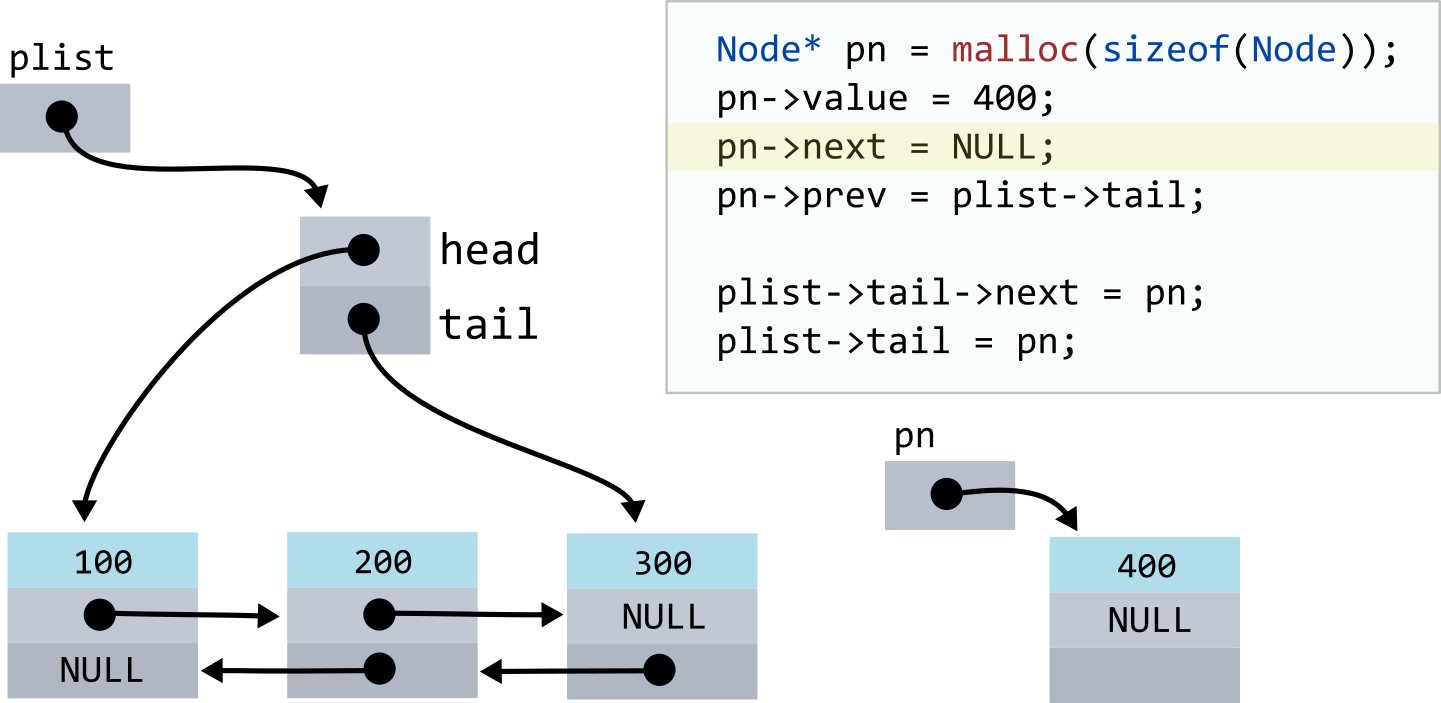
\includegraphics[width=\imageSizeMult\linewidth]{../images/doublylist/doublylist_addlast4.png}
\end{center}
\end{frame}


\begin{frame}[fragile]
\frametitle{Добавление элемент в конец двусвязного списка}
\begin{center}
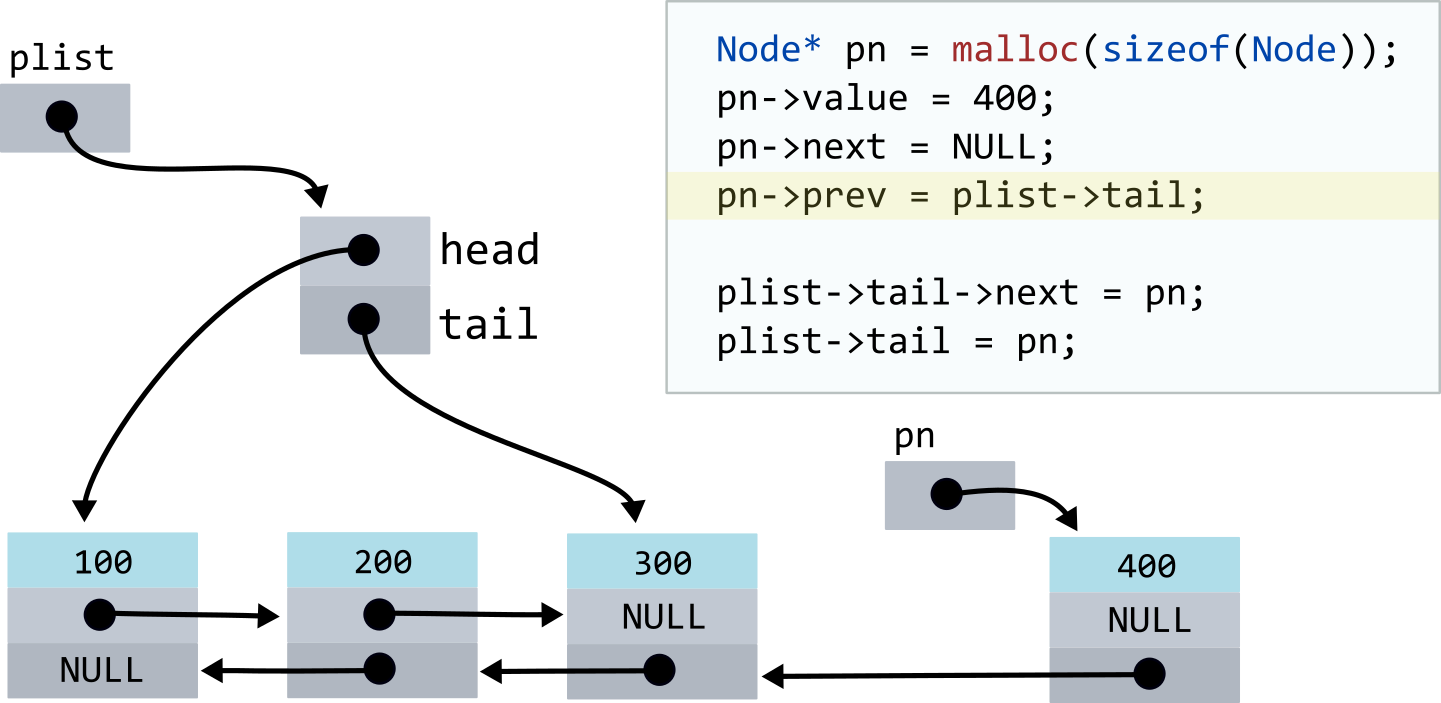
\includegraphics[width=\imageSizeMult\linewidth]{../images/doublylist/doublylist_addlast5.png}
\end{center}
\end{frame}


\begin{frame}[fragile]
\frametitle{Добавление элемент в конец двусвязного списка}
\begin{center}
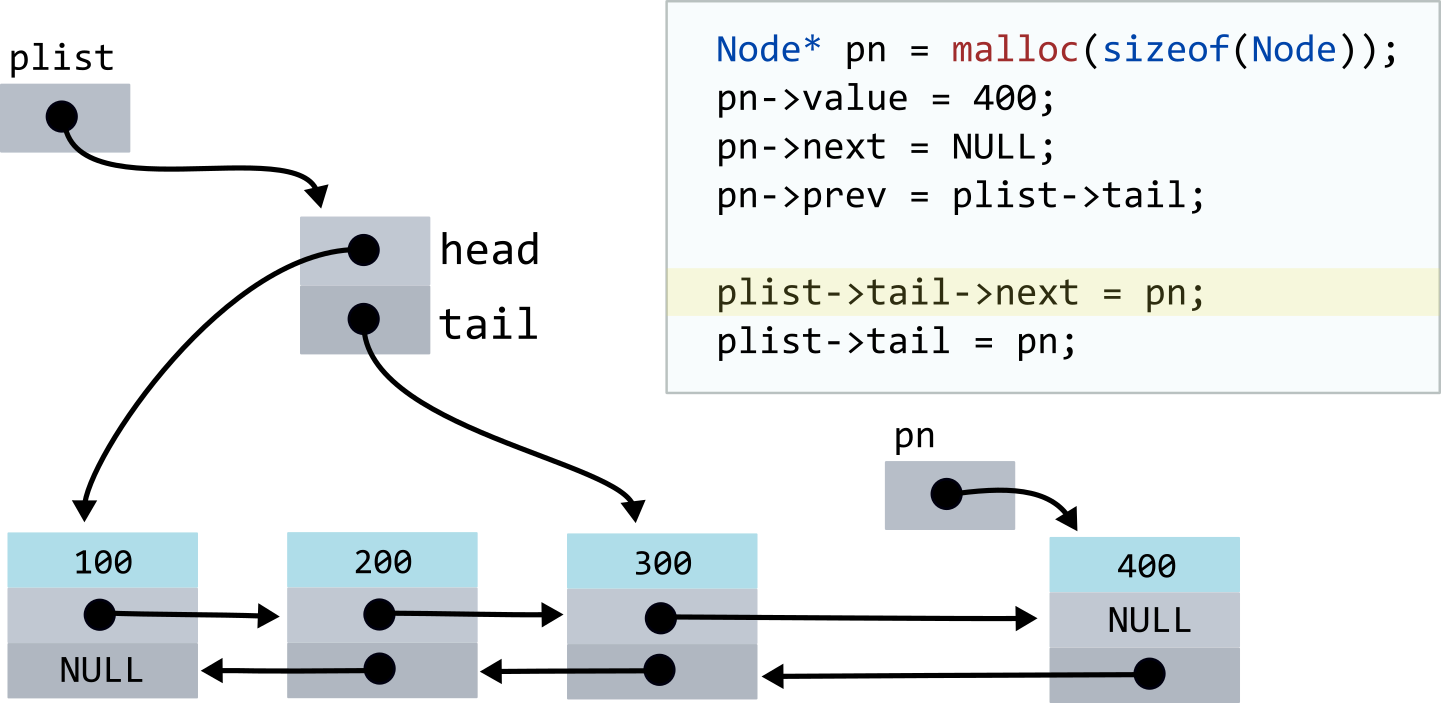
\includegraphics[width=\imageSizeMult\linewidth]{../images/doublylist/doublylist_addlast6.png}
\end{center}
\end{frame}


\begin{frame}[fragile]
\frametitle{Добавление элемент в конец двусвязного списка}
\begin{center}
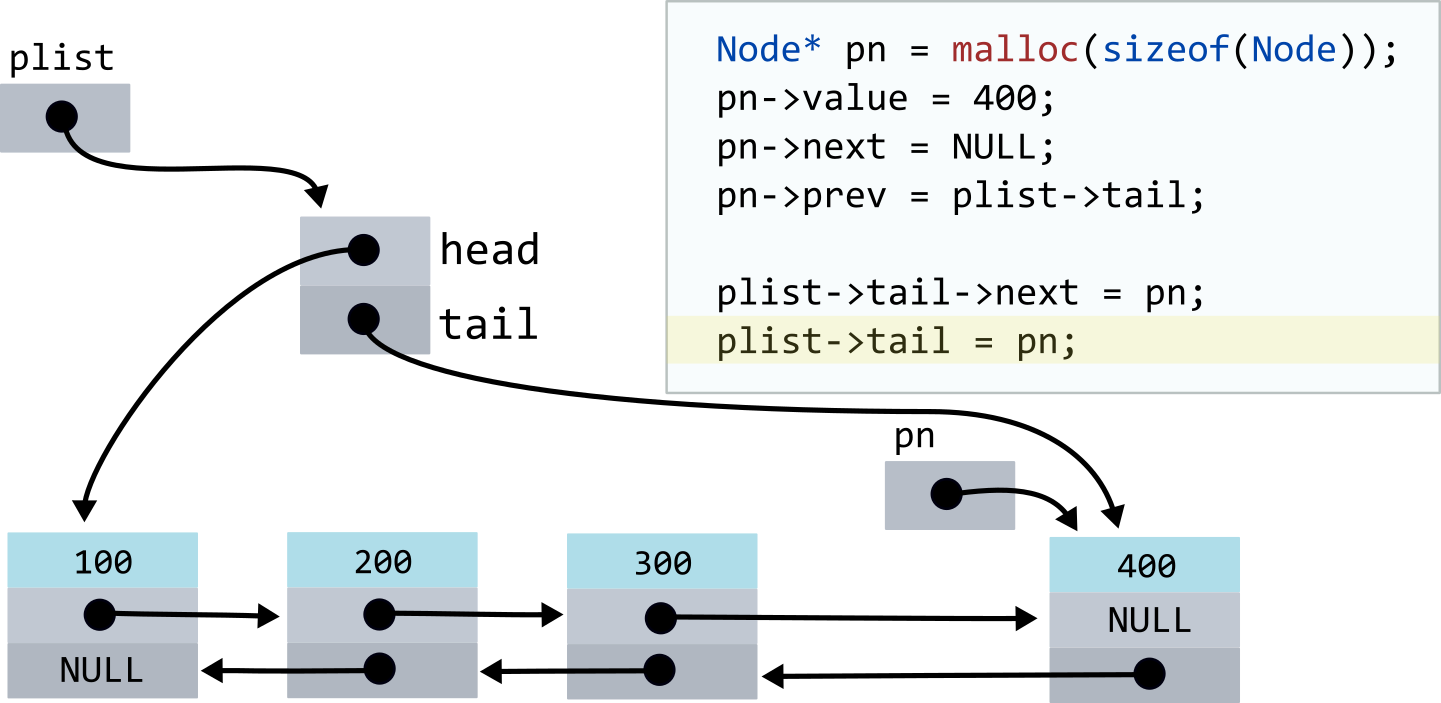
\includegraphics[width=\imageSizeMult\linewidth]{../images/doublylist/doublylist_addlast7.png}
\end{center}
\end{frame}

\begin{frame}[fragile]
\frametitle{Добавление элемент в конец двусвязного списка}
\begin{center}
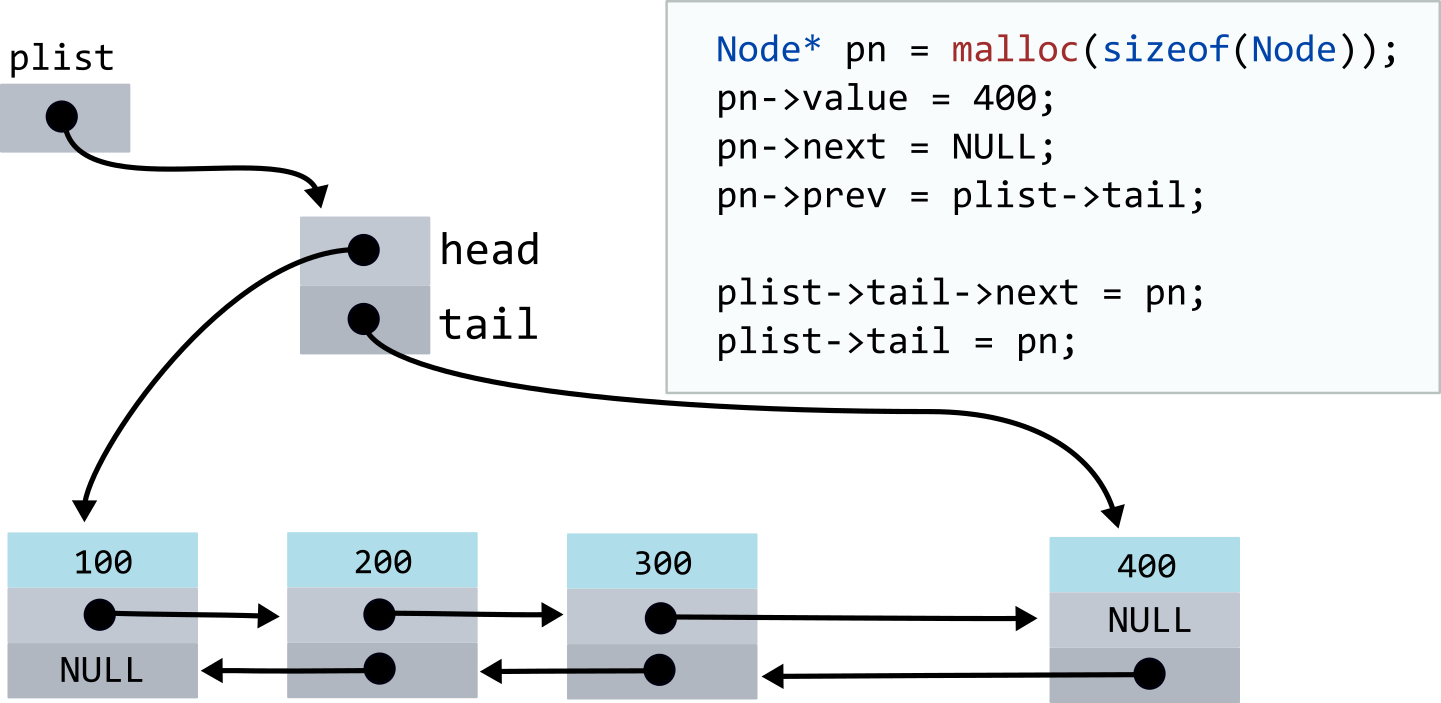
\includegraphics[width=\imageSizeMult\linewidth]{../images/doublylist/doublylist_addlast8.png}
\end{center}
\end{frame}

\section{Циклический двусвязный список}

\begin{frame}[fragile]
\frametitle{Циклический двусвязный список: Определение}
\begin{center}
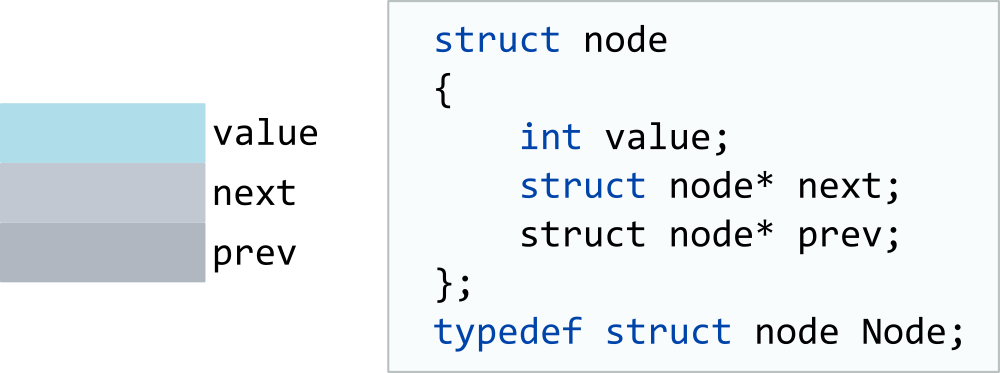
\includegraphics[width=\imageSizeMult\linewidth]{../images/doublylist/circular_doublylist_definition.png}
\end{center}
\end{frame}

\begin{frame}[fragile]
\frametitle{Циклический двусвязный список}
\begin{center}
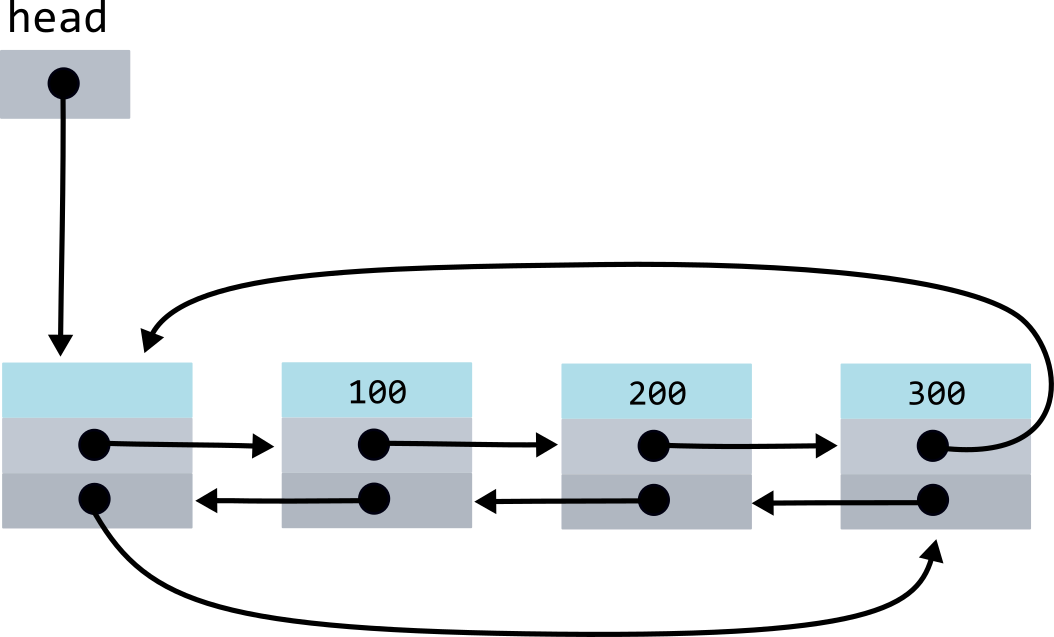
\includegraphics[width=\imageSizeMult\linewidth]{../images/doublylist/circular_list.png}
\end{center}
\end{frame}

\end{document}
